%----------------------------------------------------------------------------------
% Exemplo do uso da classe tcc.cls. Veja o arquivo .cls
% para mais detalhes e instruções.
%----------------------------------------------------------------------------------

% Seleção de idioma da monografia. Por enquanto as únicas opções
% suportadas são 'portuguese' e 'english'
% Para impressão em frente e verso, use a opção 'twoside'. Da
% mesma forma, use 'oneside' para impressão em um lado apenas.
\documentclass[portuguese,oneside]{tcc}

%----------------------------------------------------------------
% Coloque seus pacotes abaixo.
%
% Obs.: muitos pacotes de uso comum do LaTeX, como amsmath,
% geometry e url já são automaticamente incluídos pela classe
% (veja o arquivo .cls). Isso torna obrigatória a presença destes
% no sistema para o uso desta classe, mas ao mesmo tempo o uso se
% torna mais simples.  Recomendo a instalação da versão mais
% recente da distribuição TeXLive (para Windows e UNIXes):
% www.tug.org/texlive/
%
% Pacotes e opções já incluídas automaticamente:
%
% \RequirePackage[T1]{fontenc}[2005/09/27]
% \RequirePackage[utf8x]{inputenc}[2008/03/30]
% \RequirePackage[english,brazil]{babel}[2008/07/06]
% \RequirePackage[a4paper]{geometry}[2010/09/12]
% \RequirePackage{textcomp}[2005/09/27]
% \RequirePackage{lmodern}[2009/10/30]
% \RequirePackage{indentfirst}[1995/11/23]
% \RequirePackage{setspace}[2000/12/01]
% \RequirePackage{textcase}[2004/10/07]
% \RequirePackage{float}[2001/11/08]
% \RequirePackage{amsmath}[2000/07/18]
% \RequirePackage{amssymb}[2009/06/22]
% \RequirePackage{amsfonts}[2009/06/22]
% \RequirePackage{url}
% \RequirePackage[table]{xcolor}[2007/01/21]
%----------------------------------------------------------------
% Para inserção de figuras.
\usepackage{graphicx}
\graphicspath{ {images/} }
%\usepackage{longtable}


%TABLE
\usepackage[table]{xcolor} 
\setlength{\tabcolsep}{15pt}
\renewcommand{\arraystretch}{1.0}
 
\usepackage[rightcaption]{sidecap}
\usepackage{wrapfig}
%sections
\setcounter{tocdepth}{2}
% Utilize a opção 'pdftex' se você estiver usando o pdflatex (que
% permite figuras em formatos como .jpg ou .png)
%\usepackage[pdftex]{graphicx}

% Para tabelas com elementos ocupando mais de uma linha
\usepackage{multirow}
% Para frações na mesma linha (ex. ⅓).
\usepackage{nicefrac}

%Includes "References" in the table of contents
\usepackage[nottoc]{tocbibind}
\usepackage{array}
\usepackage{pgfgantt}
\usepackage{tabularx}

\usepackage{amsmath,amsfonts,amssymb,amsthm}
\usepackage{booktabs}
%\reversemarginpar

\usepackage{caption}
\usepackage{marginnote}

% Para inserir figuras lado a lado.
% \usepackage{subfigure}
% Para formatar algoritmos.
% A opção [algo2e] é necessária para evitar conflitos
% com as definições da classe.
%\usepackage[algo2e]{algorithm2e}
\usepackage{algorithmic}
% Um float do tipo algoritmo. No momento
% este pacote é incompatível com a classe.
%\usepackage{algorithm}

%----------------------------------------------------------------
% Autor (OBRIGATÓRIO)
%----------------------------------------------------------------
\author{Eduardo Ouriques \linebreak  Vicente Miraber}

%----------------------------------------------------------------
% Título (OBRIGATÓRIO). Devem ser passados DOIS parâmetros,
% o título em português E o inglês, não importando o idioma
% escolhido. Os títulos são utilizados para a montagem da capa,
% resumo e abstract mais tarde.
%----------------------------------------------------------------
\title{FLORENCE: Software para captação e doação de órgãos e tecidos}
      {FLORENCE: Software for capture and donation of organs and tissues}

%----------------------------------------------------------------
% Opções para o tipo de trabalho (OBRIGATÓRIO)
%----------------------------------------------------------------
%\tipotrabalho{\ptci}         % Proposta de Trabalho de Conclusão
\tipotrabalho{\tci}         % Trabalho de Conclusão I
%\tipotrabalho{\tcii}        % Trabalho de Conclusão II

%----------------------------------------------------------------
% Seleção do curso ("este trabalho é um requisito parcial para
% obtenção do grau de (mestre ou doutor) em Ciência da Computação").
%----------------------------------------------------------------
%\curso{\cc} % Ciência da Computação
\curso{\si} % Sistemas de Informação
%\curso{\es} % Engenharia de Software

%----------------------------------------------------------------
% Orientador (e Co-orientador, caso haja um). É OBRIGATÓRIO
% informar pelo menos o orientador.
%----------------------------------------------------------------
\orientador{Tiago Ferreto}
%\coorientador{Ciclano de Farias}

%----------------------------------------------------------------
% A capa é inserida automaticamente. Por isso não é necessário
% chamar \maketitle
%----------------------------------------------------------------
\begin{document}

%----------------------------------------------------------------
% Depois da capa vem a dedicatória e a epígrafe.
%----------------------------------------------------------------
%\dedicatoria{Dedico este trabalho a meus pais.}

%\epigrafe{The art of simplicity is a puzzle of complexity.}
      %   {Douglas Horton}

%----------------------------------------------------------------
% Também dá para fazer as duas na mesma página:
%----------------------------------------------------------------
%\dedigrafe{Dedico este trabalho a meus pais.}
%          {The art of simplicity is a puzzle of complexity.}
%          {Douglas Horton}

%----------------------------------------------------------------
% A seguir, a página de agradecimentos (OPCIONAL):
%----------------------------------------------------------------
%\begin{agradecimentos}

%Agradecemos todas aquelas pessoas envolvidas nesta etapa universitária tal como família família e amigos.

%\end{agradecimentos}

%----------------------------------------------------------------
% Resumo, com as palavras-chave passadas por parâmetro
% (OBRIGATÓRIO, ao menos para teses e dissertações)
%----------------------------------------------------------------
\begin{resumo}{doação de ógãos, computação móvel, computação em nuvem, segurança}
O processo de doação e captação de órgãos ou tecidos inicia com o diagnóstico de óbito por morte encefálica ou parada cardíaca. Atualmente a comunicação entre as Organizações de Procura de Órgãos (OPO), Comissões Intra-Hospitalares de Doação de Órgãos e Tecidos para Transplantes (CIHDOTT) e Centrais Regionais de Transplante (CRT) ocorre de maneira rudimentar, com o uso do telefone, fax ou prontuários impressos. Este trabalho de conclusão tem como objetivo desenvolver um software para reduzir o tempo gasto no processo, centralizar a comunicação em um aplicativo móvel conectado ao software e melhorar a segurança dos dados dos pacientes.

\sigla{OPO}{Organização de Procura de Órgãos}
\sigla{CIHDOTT}{Comissão Intra-Hospitalares de Doação de Órgãos e Tecidos para Transplantes}
\sigla{CRT}{Central Regional de Transplante}

\end{resumo}

%----------------------------------------------------------------
% Abstract, com as palavras-chave passadas por parâmetro
% (OBRIGATÓRIO, ao menos para teses e dissertações)
%----------------------------------------------------------------
\begin{abstract}{organ donation, mobile computing, cloud computing, security}

The process of organ and tissues donation starts with a diagnosis of encephalic death or cardiac rest. Nowadays the communication between organizations of organ searching (OPO), Intra-Hospital Commissions for Organ Donation and Tissues for Transplants (CIHDOTT) and Regional Transplant Centers (CRT) works rudimentary by phone, fax or printed reports. This final paper has the goal of developing a software to reduce the spending time by the process, centralize the communication in a mobile application connected to the software and improve the patient’s data security.
\end{abstract}

%----------------------------------------------------------------
% Listas e sumário, nessa ordem. Somente o sumário é obrigatório,
% portanto, comente as outras listas, caso sejam desnecessárias.
%----------------------------------------------------------------
\listoffigures       % Lista de figuras      (OPCIONAL)
\listoftables        % Lista de tabelas      (OPCIONAL)
%\listofalgorithms    % Lista de algoritmos   (OPCIONAL)
\listofacronyms      % Lista de siglas       (OPCIONAL)
%\listofabbreviations % Lista de abreviaturas (OPCIONAL)
%\listofsymbols       % Lista de símbolos     (OPCIONAL)
\tableofcontents     % Sumário               (OBRIGATÓRIO)

%----------------------------------------------------------------
% Aqui começa o desenvolvimento do trabalho. Para uma melhor
% organização do documento, separe-o em arquivos,
% um para cada capítulo. Para isso, utilize o comando \include,
% como mostrado abaixo.
%----------------------------------------------------------------
%\include{fundamentacao-teorica}
%\include{estado-da-arte}
%\include{proposta-do-trabalho}
%\include{cronograma-e-recursos-necessarios}

%----------------------------------------------------------------
% Após \appendix, se iniciam os capítulos de Apêndice, com
% numeração alfabética.
%----------------------------------------------------------------
\chapter{Introdução}
O processo de doação e captação de órgãos no Brasil segue uma combinação dos modelos norte-americano e espanhol, pois conta com as comissões intra-hospitalares, como a Espanha, mas também tem as Organizações de Procura de Órgãos (OPO), tipicamente norte-americanas.
%%%\cite{alberteinsten}

Conforme a Portaria nº 2.601, de 21 de outubro de 2009, entende-se por Organização de Procura de Órgãos e Tecidos (OPO), a organização com papel de coordenação supra hospitalar, responsável por organizar e apoiar, no âmbito de sua atuação e em conformidade com o estabelecido no Regulamento Técnico do Sistema Nacional de Transplantes, as atividades relacionadas ao processo de doação de órgãos e tecidos.

Outras atividades também são de responsabilidade da OPO, tais como manutenção de possível doador, a identificação e a busca de soluções para as fragilidades do processo, a construção de parcerias, o desenvolvimento de atividades de trabalho e a capacitação para identificação e efetivação da doação de órgãos ou tecidos \cite{PORTALDASAUDEOPO}. 
%http://portalsaude.saude.gov.br/index.php/o-ministerio/principal/secretarias/972-sas-raiz/dahu-raiz/transplantes-raiz/snt-2/snt-2-linha-2/21298-organizacao-de-procura-de-orgaos

Na abordagem americana, as OPO's são responsáveis por um número variável e pré determinado de hospitais de pequeno porte, os quais são incapazes de inicializar e terminar um processo de doação. %%%\cite{fernandofigueira}

Na abordagem europeia, a portaria 1.752/2005 determina a constituição de Comissão Intra-Hospitalar de Doação de Órgãos e Tecidos para Transplante (CIHDOTT) em todos os hospitais públicos, privados e filantrópicos com mais de 80 leitos \cite{PORTALDASAUDEOPO}. 
%http://portalsaude.saude.gov.br/index.php/o-ministerio/principal/secretarias/972-sas-raiz/dahu-raiz/transplantes-raiz/snt-2/snt-2-linha-2/21298-organizacao-de-procura-de-orgaos


Entende-se por CIHDOTT, Comissão Intra-Hospitalar de Doação de Órgãos e Tecidos para Transplantes, responsável por identificar possíveis doadores de órgãos.

A recusa familiar representa um grande entrave à realização dos transplantes, contribuindo para que o número de doadores seja insuficiente para atender à demanda crescente de receptores em lista de espera, sendo também apontada como um dos grandes fatores responsáveis pela escassez de órgãos e tecidos para transplantes \cite{EPRECISOEDUCAR}.

%Doação de órgãos: é preciso educar para avançar

O processo de identificação de um possível doador inicia com o preenchimento de um prontuário médico. A partir do preenchimento deste prontuário a Organização de Procura de Órgãos envia um e-mail a Central Regional de Transplantes que tem a responsabilidade de monitorar possíveis doadores.

Com base em reuniões realizadas junto aos profissionais da OPO1 (Hospital São Lucas), OPO2 (Hospital Moinhos de Vento) e a Central Regional de Transplantes do Rio Grande do Sul, foi identificado um grande número de atrasos na liberação de órgãos devido a procedimentos manuais, o alto custo financeiro gerado pelo custo das ligações e a insegurança de dados dos pacientes que são guardados fisicamente dentro de salas sem restrição de acesso.

Neste trabalho será desenvolvido um software para o gerenciamento de processos de captação e doação de órgãos, a fim de acelerar e facilitar a comunicação entre os órgãos envolvidos.

Através deste software o tempo gasto para liberar a doação do órgão e o acesso aos dados dos pacientes serão reduzidos.

%\appendix
%\appendix
\chapter{Fundamentação Teórica}
Este capítulo contém a fundamentação teórica que descreve a atual organização do processo de captação de um possível doador de órgãos no Brasil, o conceito de computação na nuvem e segurança da informação.

\section{Doação de Órgãos no Brasil}

O atual sistema para maximizar a identificação de potenciais doadores de órgãos no Brasil divide-se em quatro organizações: Organização de procura de Órgãos (OPO); Comissão Intra-Hospitalar de Doação de Órgãos e Tecidos (CIHDOTT); Central Regional de Transplante; Central Nacional de Transplante (CNT).

\subsection{Organização de Procura de Órgãos - OPO}
%\subsection*{Organização de Procura de Órgãos - OPO}
A Organização de Procura de Órgãos, também conhecida como OPO, é uma organização que está vinculada diretamente à Central de Transplantes do estado e caracteriza-se por ser uma organização supra-hospitalar com o objetivo de apoiar e executar as atividades relacionadas à doação de órgãos e tecidos no Brasil.

Este órgão é responsável por realizar visitas aos hospitais, entre outras atividades a fim de identificar potenciais doadores de órgãos e apoiar a gestão do processo\cite{HOSPITALSAOLUCAS}.   %http://www.hospitalsaolucas.pucrs.br/novo_site/doacaoorgaos.php

\subsection{Comissão Intra-Hospitalar de Doação de Órgãos e Tecidos - CIHDOTT}
A Comissão Intra-Hospitalar de Doação de Órgãos e Tecidos, também chamada de CIHDOTT, consiste em uma comissão regida pela Portaria número 1262, de 16 de junho de 2006 \cite{HCI}.
Tem como objetivo a identificação de potenciais doadores que sofreram morte cerebral ou ataque cardíaco em seu hospital vigente. Fazendo a triagem e iniciar o processo de doação de órgãos em parceria com a Central Regional de Transplantes é uma das suas responsabilidades.



%\subsection*{Comissão Intra-Hospitalar de Doação de Órgãos e Tecidos - CIHDOTT}
A Comissão Intra-Hospitalar de Doação de Órgãos e Tecidos, também chamada de CIHDOTT, consiste em uma comissão regida pela Portaria nº 1262 de 16 de junho de 2006 \cite{HCI}.
%http://www.hci.org.br/site/servicos_detalhes.php?codigo=20


De acordo com a Seção II da portaria no 2.600 \cite{PORTARIA}, de 21 de outubro de 2009, existem 3 níveis de CIHDOTT conforme descrito pelo Ministério da Saúde:

CIHDOTT I: estabelecimento de saúde com até 200 (duzentos) óbitos por ano e leitos para assistência ventilatória (em terapia intensiva ou emergência), e profissionais da área de medicina interna ou pediatria ou intensivismo, ou neurologia ou neurocirurgia ou neuropediatria, integrantes de seu corpo clínico.

CIHDOTT II: estabelecimento de saúde de referência para trauma e/ou neurologia e/ou neurocirurgia com menos de 1000 (mil) óbitos por ano ou estabelecimento de saúde não-
oncológico, com 200 (duzentos) a 1000 (mil) óbitos por ano; e

CIHDOTT III: estabelecimento de saúde não-oncológico com mais de 1000 (mil) óbitos por ano ou estabelecimento de saúde com pelo menos um programa de transplante de órgão.

A criação das CIHDOTT será opcional para todos os demais hospitais que não se enquadrem nos perfis descritos nos incisos deste artigo, e deverão ser classificadas pela CNCDO Estadual ou Regional \cite{BVSMS}.

%http://bvsms.saude.gov.br/bvs/saudelegis/gm/2009/prt2600_21_10_2009.html

\subsection{Central Regional de Transplante}
%\subsection*{Central Estadual de Transplante}
A partir da aprovação do Regulamento Técnico de Transplantes, o Ministério da Saúde desenvolveu, em parceria com as Secretarias Estaduais de Saúde, um grande esforço no sentido de implantar nos estados as Centrais de Notificação, Captação e Distribuição de Órgãos (CNCDO)\sigla{CNCDO}{Central de Notificação, Captação e Distribuição de Órgãos}, também chamadas de Centrais Estaduais de Transplante \cite{SEST}. 
%http://www1.saude.rs.gov.br/wsa/portal/index.jsp?menu=servicos&cod=3085

A CNCDO é o órgão público da secretaria do estado do Rio Grande do Sul que gerencia o processo de doação de órgãos e transplantes no Estado.

A central tem atividade ininterrupta funcionando 24 horas por dia continuamente nos 7 dias da semana para cumprir suas atribuições, uma vez que o processo de transplante requer decisão e coordenação imediata \cite{SCSCT}.
%http://www.saude.rs.gov.br/lista/132/Entenda_o_Sistema_Nacional_de_Transplantes

\subsection{Central Nacional de Transplante}
%\subsection*{Central Nacional de Transplante}
%Central Nacional de Transplante
Como a atividade das Centrais Estaduais se dá no âmbito estadual e com o desenvolvimento e incremento das atividades de transplante no País, surgiu a necessidade da criação de uma estrutura que articulasse as ações interestaduais. Portanto, em 16 de agosto de 2000, foi criada a Central Nacional de Transplantes, que funciona 24 horas por dia no Aeroporto de Brasília. 

A Central Nacional articula o trabalho das Centrais Estaduais e provê os meios para as transferências de órgãos entre estados e evita os desperdícios de órgãos sem condições de aproveitamento na sua origem. 

Quando um coração é doado e retirado num estado que não realiza transplante desse órgão, o mesmo é disponibilizado para a Central Nacional que o transfere para o estado mais próximo que realiza o procedimento \cite{SCSCT}.
%http://www.saude.rs.gov.br/lista/132/

\section{Processo de Captação e Doação de Órgãos ou Tecidos} \label{tab:processo-captacao-doacao}
O processo de captação e doação de órgãos é dividido em 5 etapas \cite{EPRECISOEDUCAR} que inicia com o diagnóstico de morte encefálica de um potencial doador e termina na liberação do corpo doador.

%\subsection*{Identificação do Potencial Doador}
\paragraph*{• Etapa 1 : Identificação do Potencial Doador}

A identificação de um possível doador com morte encefálica se dá através do preenchimento de um formulário, criado em parceria pelas OPO’s estaduais, com informações pessoais e clínicas.

O primeiro exame é realizado para verificar se o paciente não possui mais reflexo cerebral e o outro para diagnosticar a incapacidade de respirar sozinho. Estes exames são realizados em um período pré determinado de horas, dependendo da idade do paciente. 

Após realizar os primeiros exames a Central de Transplantes é notificada e então inicia o monitoramento do processo em questão.

\paragraph*{• Etapa 2 : Seleção do Receptor}
%\subsection*{Seleção do Receptor}
O processo de seleção dos receptores é feito de forma anônima; Nunca um receptor pode saber quem foi seu doador e vice-versa. O órgão a ser doado é inserido no sistema e através de suas características tal como idade do doador, tipo sanguíneo e demais informações relevantes; Uma lista de possíveis receptores é gerada e organizada por compatibilidade.

\paragraph*{• Etapa 3 : Identificação da Equipe Transplantadora}
%\subsection*{Identificação da Equipe Transplantadora}
Após a seleção do receptor, a Central Regional de Transplantes notifica a equipe de transplantes responsável pelo paciente que dá início ao processo de retirada dos órgãos do doador.

\paragraph*{• Etapa 4 : Retirada dos Órgãos}
%\subsection*{Retirada dos Órgãos}
A equipe notificada pela Central Regional de Transplantes se dirige ao hospital onde o doador está internado e inicia o processo da retirada do órgão; Terminado o processo, a equipe se dirige ao hospital do receptor e começa o processo de transplante.

\paragraph*{• Etapa 5 : Liberação do Corpo}
%\subsection*{Liberação do Corpo}
Após a retirada dos órgãos o doador passa por um processo de recomposição para então ser entregue a família.


\section{Detalhamento da Atual Organização dos Processos}  \label{tab:detalhamento-atual}
Esta seção tem como objetivo descrever detalhadamente o atual processo de doação de órgãos no Brasil descrito no capítulo \ref{tab:processo-captacao-doacao}, e como seus atores interagem para concluir o processo de doação com a maior eficácia possível.


\begin{figure}[htp]
\centering
\caption{Atual Organização dos Processos}
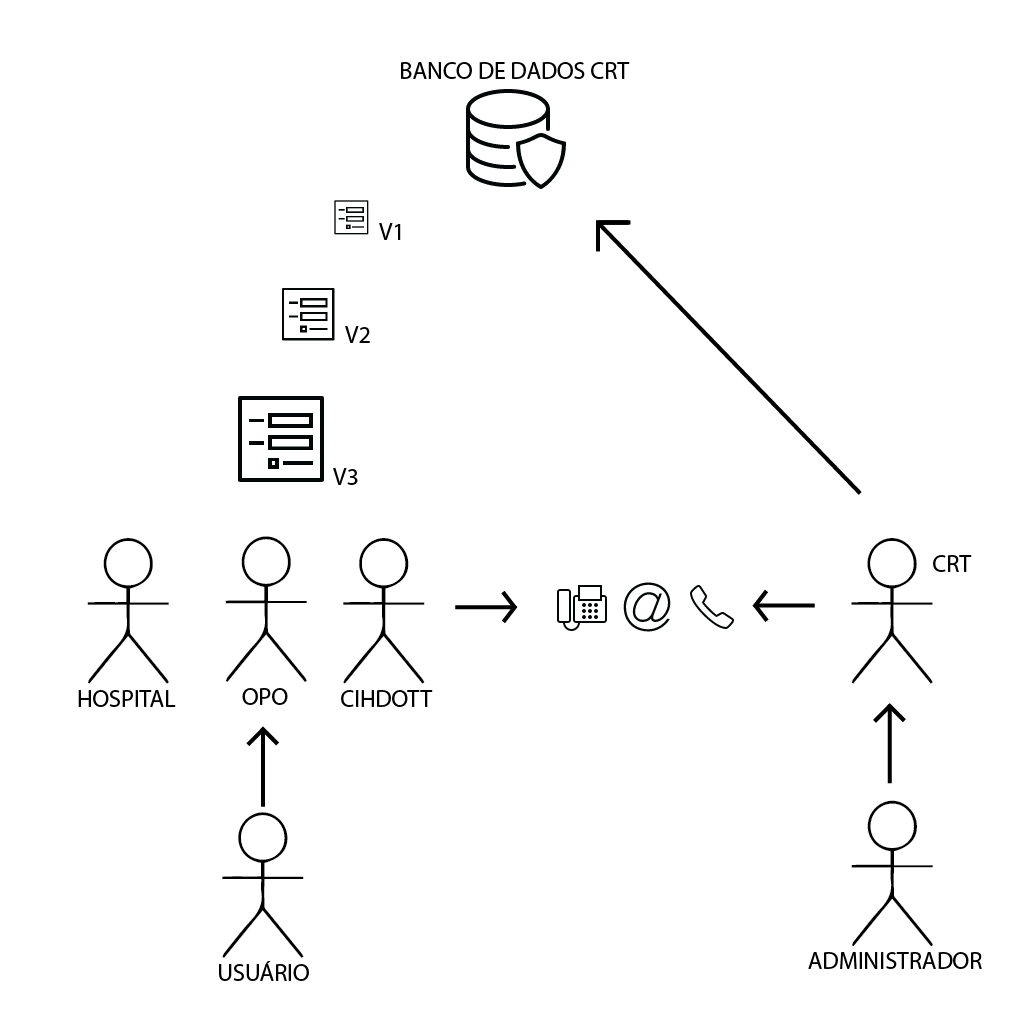
\includegraphics[width=10cm]{processo-rudimentar}

\label{fig:processo-rudimentar}
\end{figure}


\begin{enumerate}

\item O ator identifica um possível doador.
\item O ator da abertura em um prontuário de papel e o preenche (V1).
\item O ator  tem dificuldades para preencher algumas informações e solicita auxílio da OPO.

\item O ator OPO se dirige ao hospital e o auxilia a preencher o restante do prontuário.

\item O ator OPO faz o primeiro exame necessário junto com o Ator responsável.

\item A OPO envia o prontuário para a CRT (V2) via e-mail.

\item A Central Regional de Transplantes dá início ao monitoramento deste processo.

\item A Central Regional de Transplantes percebe a demora fora do comum para o recebimento do prontuário o qual contém o resultado do segundo exame e entra em contato com a OPO responsável.

\item A OPO entra em contato com o ator responsável e envia o segundo exame (V3). 

\item A Central Regional de Transplantes verifica o exame.

\item A Central Regional de Transplantes constata que o paciente está apto para retirada dos órgãos.

\item A equipe de transplante efetua todos os transplantes dos órgãos doados.

\item O corpo do paciente é liberado para a família.

\item A Central Regional de Transplantes conclui o processo e arquiva o prontuário.
\end{enumerate}

%\subsection{Como funciona}
%Quando um potencial doador é detectado o responsável pelo mesmo preenche um formulário com informações pessoais e clínicas do paciente. O formulário é enviado por fax ou e-mail e a central de transplantes é notificada pelo responsável para dar início ao monitoramento deste processo.

%O problema começa quando novos dados começam a ser inseridos por parte do responsável ou a CRT solicita correções nos dados previamente preenchidos, seja por não preenchimento de dados obrigatórios ou erro causado pela falta de conhecimento do profissional responsável. 

%Toda a informação atualmente é trocada via email, fax ou telefone. O que acarreta na rápida perda de rastreabilidade do formulário por causa das inúmeras versões geradas pelas mudanças e falta de versionamento do mesmo. Gerando assim inconsistência nos dados dos formulários, o que implica diretamente na latência do mesmo e em altos custos com comunicação. 



%\subsection{Simulação do Processo}



\section{Análise do Processo Atual} \label{tab:detalhamento-problema}
Analisando as informações providas em reuniões com as entidades envolvidas no processo de doação de órgãos no Rio Grande do Sul, foi identificado que o problema mais grave e causador do maior impacto da demora do processo, podendo até mesmo comprometê-lo, é a falta de consistência dos dados do prontuário de doação. 

Quando um enfermeiro ou médico responsável pelo potencial doador abre um processo, ele preenche o prontuário com as informações pessoais e clínicas do paciente. 

Esse documento existe em cópia única em suas mãos, porém todas estas informações devem ser transmitidas para a Central de Transplante Regional.

Nesse exato momento de troca de informação as informações começam a ser duplicadas e alteradas, pois são transmitidas de maneira rudimentar e sem qualquer controle de versão tais como e-mail, fax ou telefone.

Atualmente, garantir unicidade e consistência dos dados é um desafio entre as entidades, o impacto da perda dos dados é muito grande e causa uma comunicação excessiva para revalidar e repreencher campos requeridos. 

Uma estratégia para resolver estes problemas é centralizar a informação em um software que auxilie no processo, com restrição de acesso a fim de evitar a exposição dos dados dos pacientes.

%Estes fatos implicam diretamente no custo do processo e em sua duração, dado que muitas doações não ocorrem porque as famílias não querem aguardar este tempo.
%\section{Tempo gasto na captação e doação de órgãos}
%\section{Alto custo financeiro de ligações}
%\section{Insegurança dos dados dos pacientes}
%\appendix


\section{Computação na Nuvem}
A computação em nuvem é um modelo para permitir acesso de rede conveniente, sob demanda a um grupo compartilhado de recursos configuráveis de computação (por exemplo, redes, servidores, armazenamento, aplicativos e serviços) que podem ser rapidamente provisionados e lançados com o mínimo de esforço \cite{NIST}.

Esta seção descreve algumas características da computação em nuvem tais como Serviço Sob Demanda; Acesso Amplo de Rede; Agrupamento de Recursos; Elasticidade Rápida; Serviços Sob Medida.

\paragraph*{• Serviço Sob Demanda}
O modelo em nuvem pode suprir capacidades de computação unilateralmente, como tempo de servidor e armazenamento de rede, conforme demanda, sem necessidade de interação humana com cada provedor de serviços.

\paragraph*{• Acesso Amplo de Rede}
Os recursos estão disponíveis através da rede e acessadas através de mecanismos padrão que promovem o uso por plataformas de clientes heterogêneos (por exemplo, telefones celulares, tablets, laptops e estações de trabalho).

\paragraph*{• Agrupamento de Recursos}
Os recursos de computação da nuvem são agrupados para atender a vários consumidores, com diferentes recursos físicos e virtuais atribuídos dinamicamente de acordo com a demanda do consumidor.

\paragraph*{• Elasticidade Rápida}
As capacidades podem ser provisionadas e liberadas elasticamente, em alguns casos automaticamente, para escalar rapidamente em conformidade com a demanda.
Para o consumidor, as capacidades disponíveis para configuração e instalação muitas vezes parecem ser ilimitadas e podem ser apropriadas em qualquer quantidade a qualquer momento.

\paragraph*{• Serviço Medido}
O uso de recursos (por exemplo, armazenamento, processamento e largura de banda) pode ser monitorado, controlado e reportado, proporcionando transparência tanto para o provedor como para o consumidor do serviço utilizado.

\section{Modelos de Implantação na Nuvem}
Esta seção descreve os principais modelos de implantação na nuvem, a fim de oferecer um melhor entendimento das características de cada uma delas. 

\section{Nuvem Privada}
Nuvem privada refere-se aos serviços de computação em nuvem oferecidos pela Internet ou por uma rede interna privada somente a usuários selecionados e não ao público geral.

As nuvens privadas oferecem um maior nível de segurança e privacidade por meio de firewalls da empresa e hosting interno para garantir que as operações e dados confidenciais não possam ser acessados por terceiros \cite{OQUEENUVEM}.

\section{Nuvem Pública}
Em uma nuvem pública, a infra-estrutura pertence a uma  organização que vende serviços para o público em geral e pode  ser acessada por qualquer usuário que conheça a localização do  serviço, não sendo admitidas técnicas de restrição de acesso ou autenticação \cite{COMPUTACAOEMNUVEM}.

As nuvens públicas tentam fornecer aos clientes elementos de  TI livres de complexidades, onde o provedor da nuvem assume  as responsabilidades de instalação, gerenciamento, disponibilização e manutenção.  

\section{Segurança da Informação}
A Sociedade Brasileira de Informática em Saúde [Oluwatosin 2006] cita a informá-tica médica ou informática em saúde como um campo de rápido desenvolvimento científico que lida com armazenamento, recuperação e uso da informação, dados estes que auxiliam na tomada de decisão dos profissionais da saúde.

Helms, Moore e Ahmadi [Helms 2008] mostra que o uso de sistemas de informa-ção na saúde oferece importantes potenciais: incremento da segurança do paciente, maior eficiência operacional e infraestrutura de TI já existente na maioria das organizações.

A privacidade e a segurança da informação no setor da saúde são pontos que requerem atenção, visto que a adoção destes sistemas estão em constante crescimento.

Portanto, este capítulo descreve dois tipos de ameaças à privacidade e a segu-rança da informação na área da saúde, conforme citado em um estudo realizado por uma escola de negócio nos Estados Unidos [Gilberto Perez 2010].


\paragraph*{• Ameaça Organizacional}
Este tipo de ameaça se refere aos acessos inapropriados aos dados dos pacien-tes pelos agentes internos que abusam dos seus privilégios ou agentes externos que se aproveitam da vulnerabilidade do sistema de informação.


\paragraph*{• Ameaça Sistêmica}
Ameaça Sistêmica se refere a um agente na cadeia de fluxo de informações dentro do processo explorando os dados divulgados além do uso pretendido, ou seja, agentes dentro das organizações da saúde que tem acesso a dados privilegiados e que por muitas vezes não possuem autorização.

\chapter{Trabalhos Relacionados}
\label{tab:trabalhos-relacionados}	
Neste capítulo estão descritos softwares relacionados ao tema deste trabalho com o objetivo de verificar níveis de segurança, e para esta análise três tópicos foram observados: criptografia; autenticação; autorização.

\section{Medware Sistemas Médicos Ltda}

\begin{figure}[htp]
\centering
\caption{Tela Principal - \textit{Medware Sistemas Médicos Ltda}}
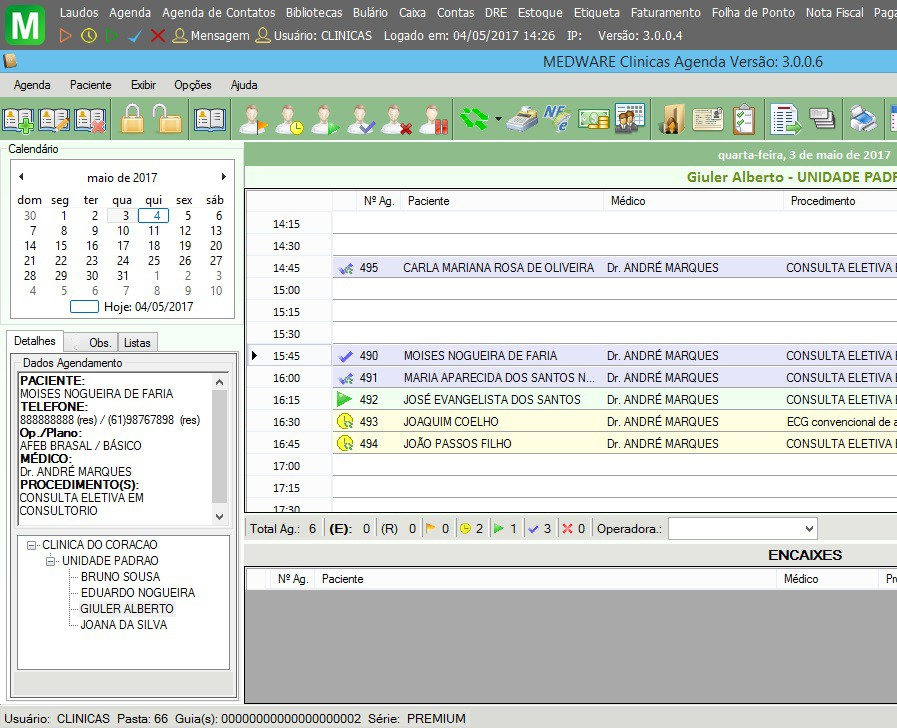
\includegraphics[width=12cm]{medware}
\label{fig:CalDoseX}
\end{figure}

A Medware Sistemas Médicos é uma empresa de desenvolvimento de sistemas voltada para a criação de soluções de informática para a área médica.

Com um rigoroso sistema de controle de qualidade e investimento em capacitação de sua equipe técnica (analistas e programadores), a Medware vem garantindo o desenvolvimento de sistemas práticos, de utilização simplificada, confiáveis e com tecnologia de ponta o que tem feito com que instituições de renome \cite{MEDWARE}.

Os prontuários seguem as recomendações do CFM e o sistema foi homologado com o nível máximo de segurança da certificação SBIS. O sistema trabalha com alguns itens de segurança tais como certificado digital, criptografia, versionamento de laudo e autenticação de usuário.

\sigla{CFM}{Conselho Federal de Medicina}

\newpage

\section{BloodSave}

\begin{figure}[htp]
\centering
\caption{Tela de Login - \textit{BloodSave}}
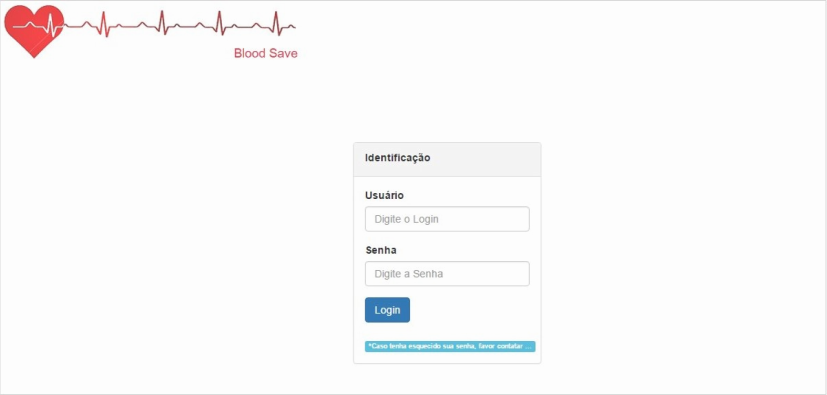
\includegraphics[width=15cm]{bloodsave}
\label{fig:bloodsave}
\end{figure}

BloodSave é um software desenvolvido para a troca e empréstimo de bolsas de hemocomponentes entre os hospitais no qual evita o desperdício \cite{SANGUE}.
 
No ponto de vista tecnológico o software demonstra certa preocupação com a exposição dos dados dos pacientes e por isso utilizou a criptografia nos dados e autenticação de usuário para melhorar o nível de segurança.

%\newpage

\section{eClinicalWorks}

\begin{figure}[htp]
\centering
\caption{Tela de Login - \textit{eClinicalWorks}}
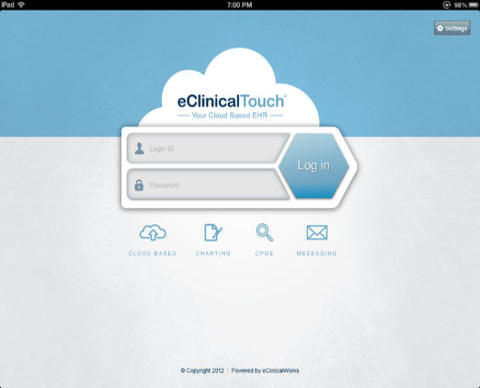
\includegraphics[width=8cm]{eclinicalworks}
\label{fig:eclinicalworks}
\end{figure}

eClinicalWorks é uma empresa de Massachusetts que vende softwares de registros médicos eletrônicos, gerenciamento de gestão e saúde \cite{ECLINICAL}.
 
O software é utilizado por diversas organizações da área da saúde e contém uma área muito ampla para gerenciamento de atividades clínicas.

Utilizando a versão free do software foi identificado uma boa preocupação de acesso aos dados, utilizando alguns mecanismos de controle de acesso, tais como autenticação e autorização.

\section{Comparação de sistema}
Para melhor entendimento, a Tabela \ref{tab:comparativo} compara os trabalhos relacionados que estão descritos no Capítulo \ref{tab:trabalhos-relacionados}, descrevendo quatro mecanismos de segurança da informação, tais como Criptografia, Autenticação, Autorização e Certificado Digital.

\paragraph{ }
\begin{table}[htb]
\caption{Tabela Comparativa de Sistemas}\label{tab:comparativo}	
	\begin{center}
	\begin{tabular}{lllll}
	\toprule
	ID & Funcionalidade & Medware Sistemas & BloodSave & eClinicalWorks\\ 
	\midrule
	1 & Criptografia 	& X	& X	&  		\\
	2 & Autenticação	& X 	& X	& X		\\
	3 & Autorização 	&  	&  	& X		\\
    4 & Certificado Digital 	& X 	&  	& X		\\
	\bottomrule
	\end{tabular}
	\end{center}
\end{table}


\paragraph*{• Criptografia}
Em relação a criptografia dos dados dos pacientes transmitidos na internet, os sistemas Medware e BloodSave apresentaram boa preocupação visto que estes sistemas criptografam os dados, diminuindo a probabilidade de quebra destes dados quando trafegados.

\paragraph*{• Autenticação}
Em relação a autenticação de usuário, os três softwares analisados apresentaram autenticação própria no sistema, ou seja, sem utilizar autenticação de sistema externo.

\paragraph*{• Autorização}
Em relação a autorização de recursos no sistema o software eClinicalWorks foi o único que apresentou preocupação garantindo que somente usuários autenticados e autorizados podem executar determinada tarefa dentro do sistema.

\paragraph*{• Certificado Digital}
Em relação a certificado digital o software da Medware segue as recomendações do Conselho Federal Médico, garantindo maior segurança na troca de informações.

\chapter{Descrição do Trabalho} \label{tab:descricao-trabalho}
Este capítulo descreve a nova organização dos processos e as definições de projeto para desenvolver o software, a fim de oferecer um melhor entendimento da arquitetura do sistema.


\section{Nova Organização dos Processos}
Conforme descrito no Capítulo \ref{tab:detalhamento-problema}, o processo atual de doação de órgãos no Brasil apresenta sérios problemas, desta forma, este trabalho visa propor um novo processo usando a tecnologia da informação.


\begin{figure}[htp]
\centering
\caption{Nova Organização dos Processos}
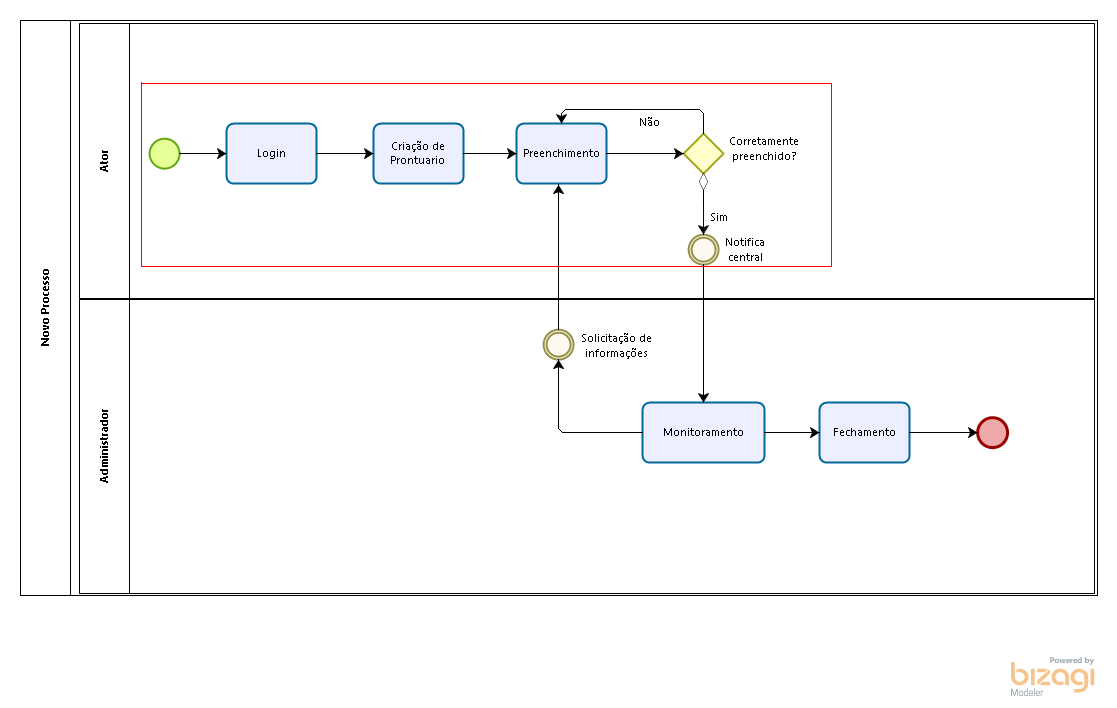
\includegraphics[width=16cm]{modelagem-novo-processo}

\label{fig:novo-processo}
\end{figure}

Assim que é identificado um potencial doador, o ator responsável - hospital, OPO ou CIHDOTT - efetua login no sistema, cria um formulário eletrônico e preenche com os dados obrigatórios.

Dado que o formulário é preenchido com todas as informações obrigatórias, um evento de notificação é gerado a Central Regional, caso contrário, o ator é notificado para preencher os dados faltantes.

Após o ator administrador ser notificado, neste caso a Central Regional, ele realiza o monitoramento dos processos e se necessário solicita novas informações do paciente.

O fechamento do processo é dado após a atualização realizada pelo administrador responsável.

\section{Objetivo}
Esta seção descreve o objetivo geral e os objetivos específicos do software de captação e doação de órgãos.


\subsection{Objetivo Geral}
Este trabalho tem como objetivo o desenvolvimento de uma plataforma de comunicação para as entidades envolvidas no processo de doação de órgãos. Provendo às mesmas, a capacidade de acessarem prontuários consistentes e identificar as falhas no processo através de gráficos e métricas, diminuindo a duração do processo e aumentando sua eficácia para salvar mais vidas.


\subsection{Objetivo Específico}
Este capítulo descreve os objetivos específicos do software de captação e doação de órgãos.

\paragraph*{• Redução da latência do processo}

Redução no tempo total do processo, desde a abertura do prontuário feita pelo responsável do paciente, até a conclusão do processo de doação quando o paciente é encaminhado para retirada dos órgãos.

\paragraph*{• Aumento na consistência das informações}

O aumento de consistência do prontuário se dará pela criação de um prontuário eletrônico e único que estará acessível para todos envolvidos em sua mais recente versão através da plataforma.

\paragraph*{• Redução de gastos com comunicação}

Através da informatização do prontuário, os gastos com comunicação serão reduzidos como consequência do aumento de acessibilidade e consistência do mesmo.

\paragraph*{• Aumento de segurança da informação}

Os dados dos pacientes que atualmente circulam por meio de fax, email, e outros meios não encriptados, agora serão encapsulados em um canal encriptado de comunicação provido pela plataforma.

\paragraph*{• Agilidade e portabilidade agregada ao processo}

O formulário anteriormente massante e extenso de ser preenchido, agora será modelado através de técnicas de desenvolvimento de interfaces humano computador e experiência de usuário, para melhor atender os responsáveis pelo preenchimento do formulário.

\paragraph*{• Geração de métricas}

Através do histórico de mudanças do formulário gerado pela plataforma, a mesma será capaz de prover métricas, facilitando a identificação de gargalos no processo e eliminação dos mesmos.

\section{Proposta de Arquitetura}

\begin{figure}[htp]
\centering
\caption{Arquitetura do software}
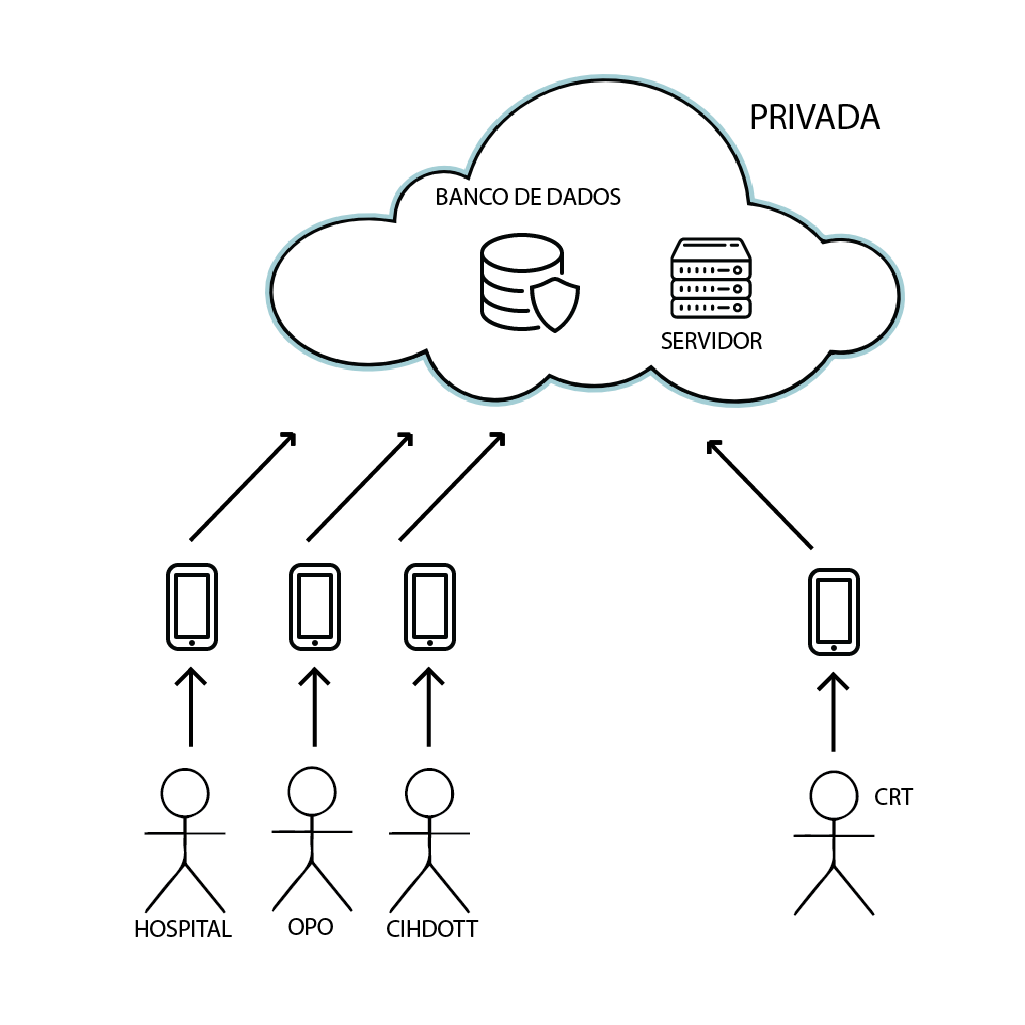
\includegraphics[width=7cm]{cliente-servidor}
\label{fig:cliente-servidor}
\end{figure}

A figura \ref{fig:cliente-servidor} mostra a arquitetura do software baseada em camadas Cliente-Servidor, tal que a camada cliente é representada pelos atores - HOSPITAL, OPO E CIHDOTT - com seus \textit{smartphones} e a camada Servidor é representada por uma nuvem privada que contém o banco de dados e o servidor.


\section{Modelo de Implantação}
Para garantir melhor segurança aos dados dos pacientes uma nuvem privada será instalada e configurada em um servidor local, onde somente os usuários autenticados e autorizados poderão consumir os serviços disponíveis.


\section{Plataforma Mobile}

Para alcançar os resultados esperados na proposta de solução deste trabalho, um canal de acesso mobile a plataforma deverá ser desenvolvido. 
 
%Sugere-se um aplicativo iOS que estará disponível na Apple Store, o mesmo será responsável por acessar e modificar os prontuário eletrônicos, capacitando também o anexo imagens e documentos no mesmo. 

O aplicativo deve ser igualmente responsável por manter o sigilo e segurança dos dados referentes aos pacientes que serão armazenados criptografados no banco de dados da plataforma.

\chapter{Modelagem do Software}
Neste capítulo estão descrito todos os requisitos do software junto ao modelo de casos de uso.

\section{Requisitos Funcionais}
Através de reuniões realizadas junto aos profissionais da OPO, localizada no hospital São Lucas, foram definidos os seguintes requisitos do software.

\begin{itemize}


\item RF01: O sistema deve permitir o login dos usuários.

\item RF02: Para realizar qualquer operação o usuário precisa estar logado.

\item RF03: Após o login, o sistema deve mostrar todas as funcionalidades relacionadas ao tipo de permissão do usuário.

\item RF04: O sistema deve permitir que o usuário cadastre um novo processo de doação.

\item RF05: O sistema deve permitir que o usuário e o administrador consultem os gráficos dos processos.

%\item RF06: O sistema deve fornecer um pré-cadastro para novos usuários.

\item RF06: O sistema deve permitir que o administrador consulte todos os processos de doação.

\item RF07: O sistema deve permitir que o administrador atualize o status de todos os processos de doação.

%\item RF09: O sistema deve permitir que o administrador gerencie novos usuários previamente cadastrados.

\item RF08: O sistema deve permitir que os usuários OPO, CIHDOTT e HOSPITAL consultem todos os processos de doação sob sua responsabilidade.

\item RF09: O sistema deve permitir que os usuários OPO e CIHDOTT notifiquem a central quando necessário.

\item RF10: O sistema deve permitir que os usuários OPO, CIHDOTT e HOSPITAL atualizem todos os processos de doação sob sua responsabilidade.

\item RF11: O sistema deve enviar um e-mail a central sempre que o status do processo for atualizado para “Pronto para Central”.

\item RF12: O sistema deve permitir que todos os usuários façam upload de arquivo.

%\item RF15: O sistema deve permitir que a OPO gerencie os hospitais.

\end{itemize}


\section{Requisitos não Funcionais}

Esta seção descreve os requisitos não funcionais para desenvolver o software de captação e doação de órgãos.

\begin{itemize}

\item RNF01: Para efetuar login no sistema o usuário deve ser autenticado após fornecer seu usuário e senha.

\item RNF02: O tráfego de senha na internet deve ser criptogrado.

\item RNF03: O ator deve ser autorizado antes de realizar qualquer operação no sistema.

\item RNF04: O aplicativo deve ser compatível com smartphone.

\item RNF05: O sistema não apresentará aos usuários quaisquer dados de cunho privativo.

\end{itemize}

%\newpage

\section{Atores do Sistema}
Esta seção apresenta todos os atores do sistema, focando na hierarquia e suas permissões.

\begin{figure}[htp]
\centering
\caption{Atores do Sistema}
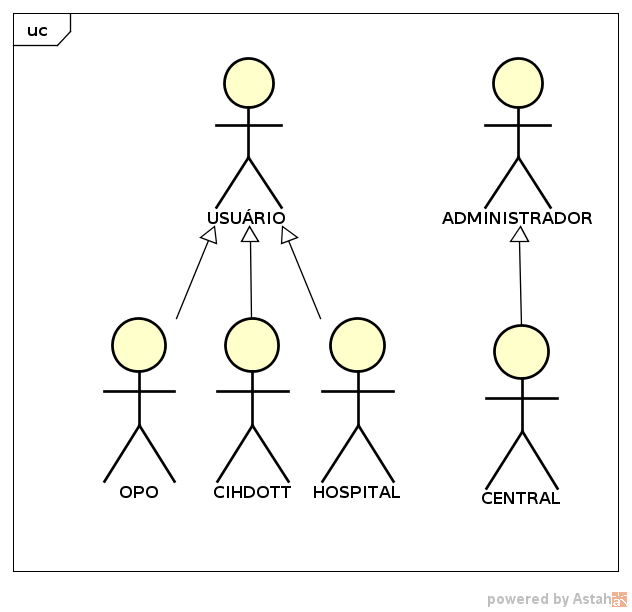
\includegraphics[width=10cm]{uc-atores}
\label{fig:uc-atores}
\end{figure}

\paragraph*{• Usuário}
O ator Usuário representa genericamente os usuários do software de captação e doação de órgão.

\paragraph*{• OPO}
O ator OPO representa os usuários da Organização de Procura de Órgãos.

\paragraph*{• CIHDOTT}
O ator CIHDOTT representa os usuários da Comissão Intra-Hospitalar de Doação de Órgãos e Tecidos para Transplantes.

\paragraph*{• Hospital}
O ator HOSPITAL representa os usuários dos hospitais.

\paragraph*{• Administrador}
O ator ADMINISTRADOR representa genericamente os usuários administradores no sistema.

\paragraph*{• Central}
O ator CENTRAL representa os usuários das centrais regionais de transplante no sistema.

\section{Casos de Uso do Sistema}
Para melhor entendimento, esta seção descreve o diagrama de Caso de Uso do sistema junto aos seus atores: Usuário; OPO; CIHDOTT; Hospital; Administrador; Central.

\paragraph{}
\begin{figure}[htp]
\centering
\caption{Diagrama de Caso de Uso}
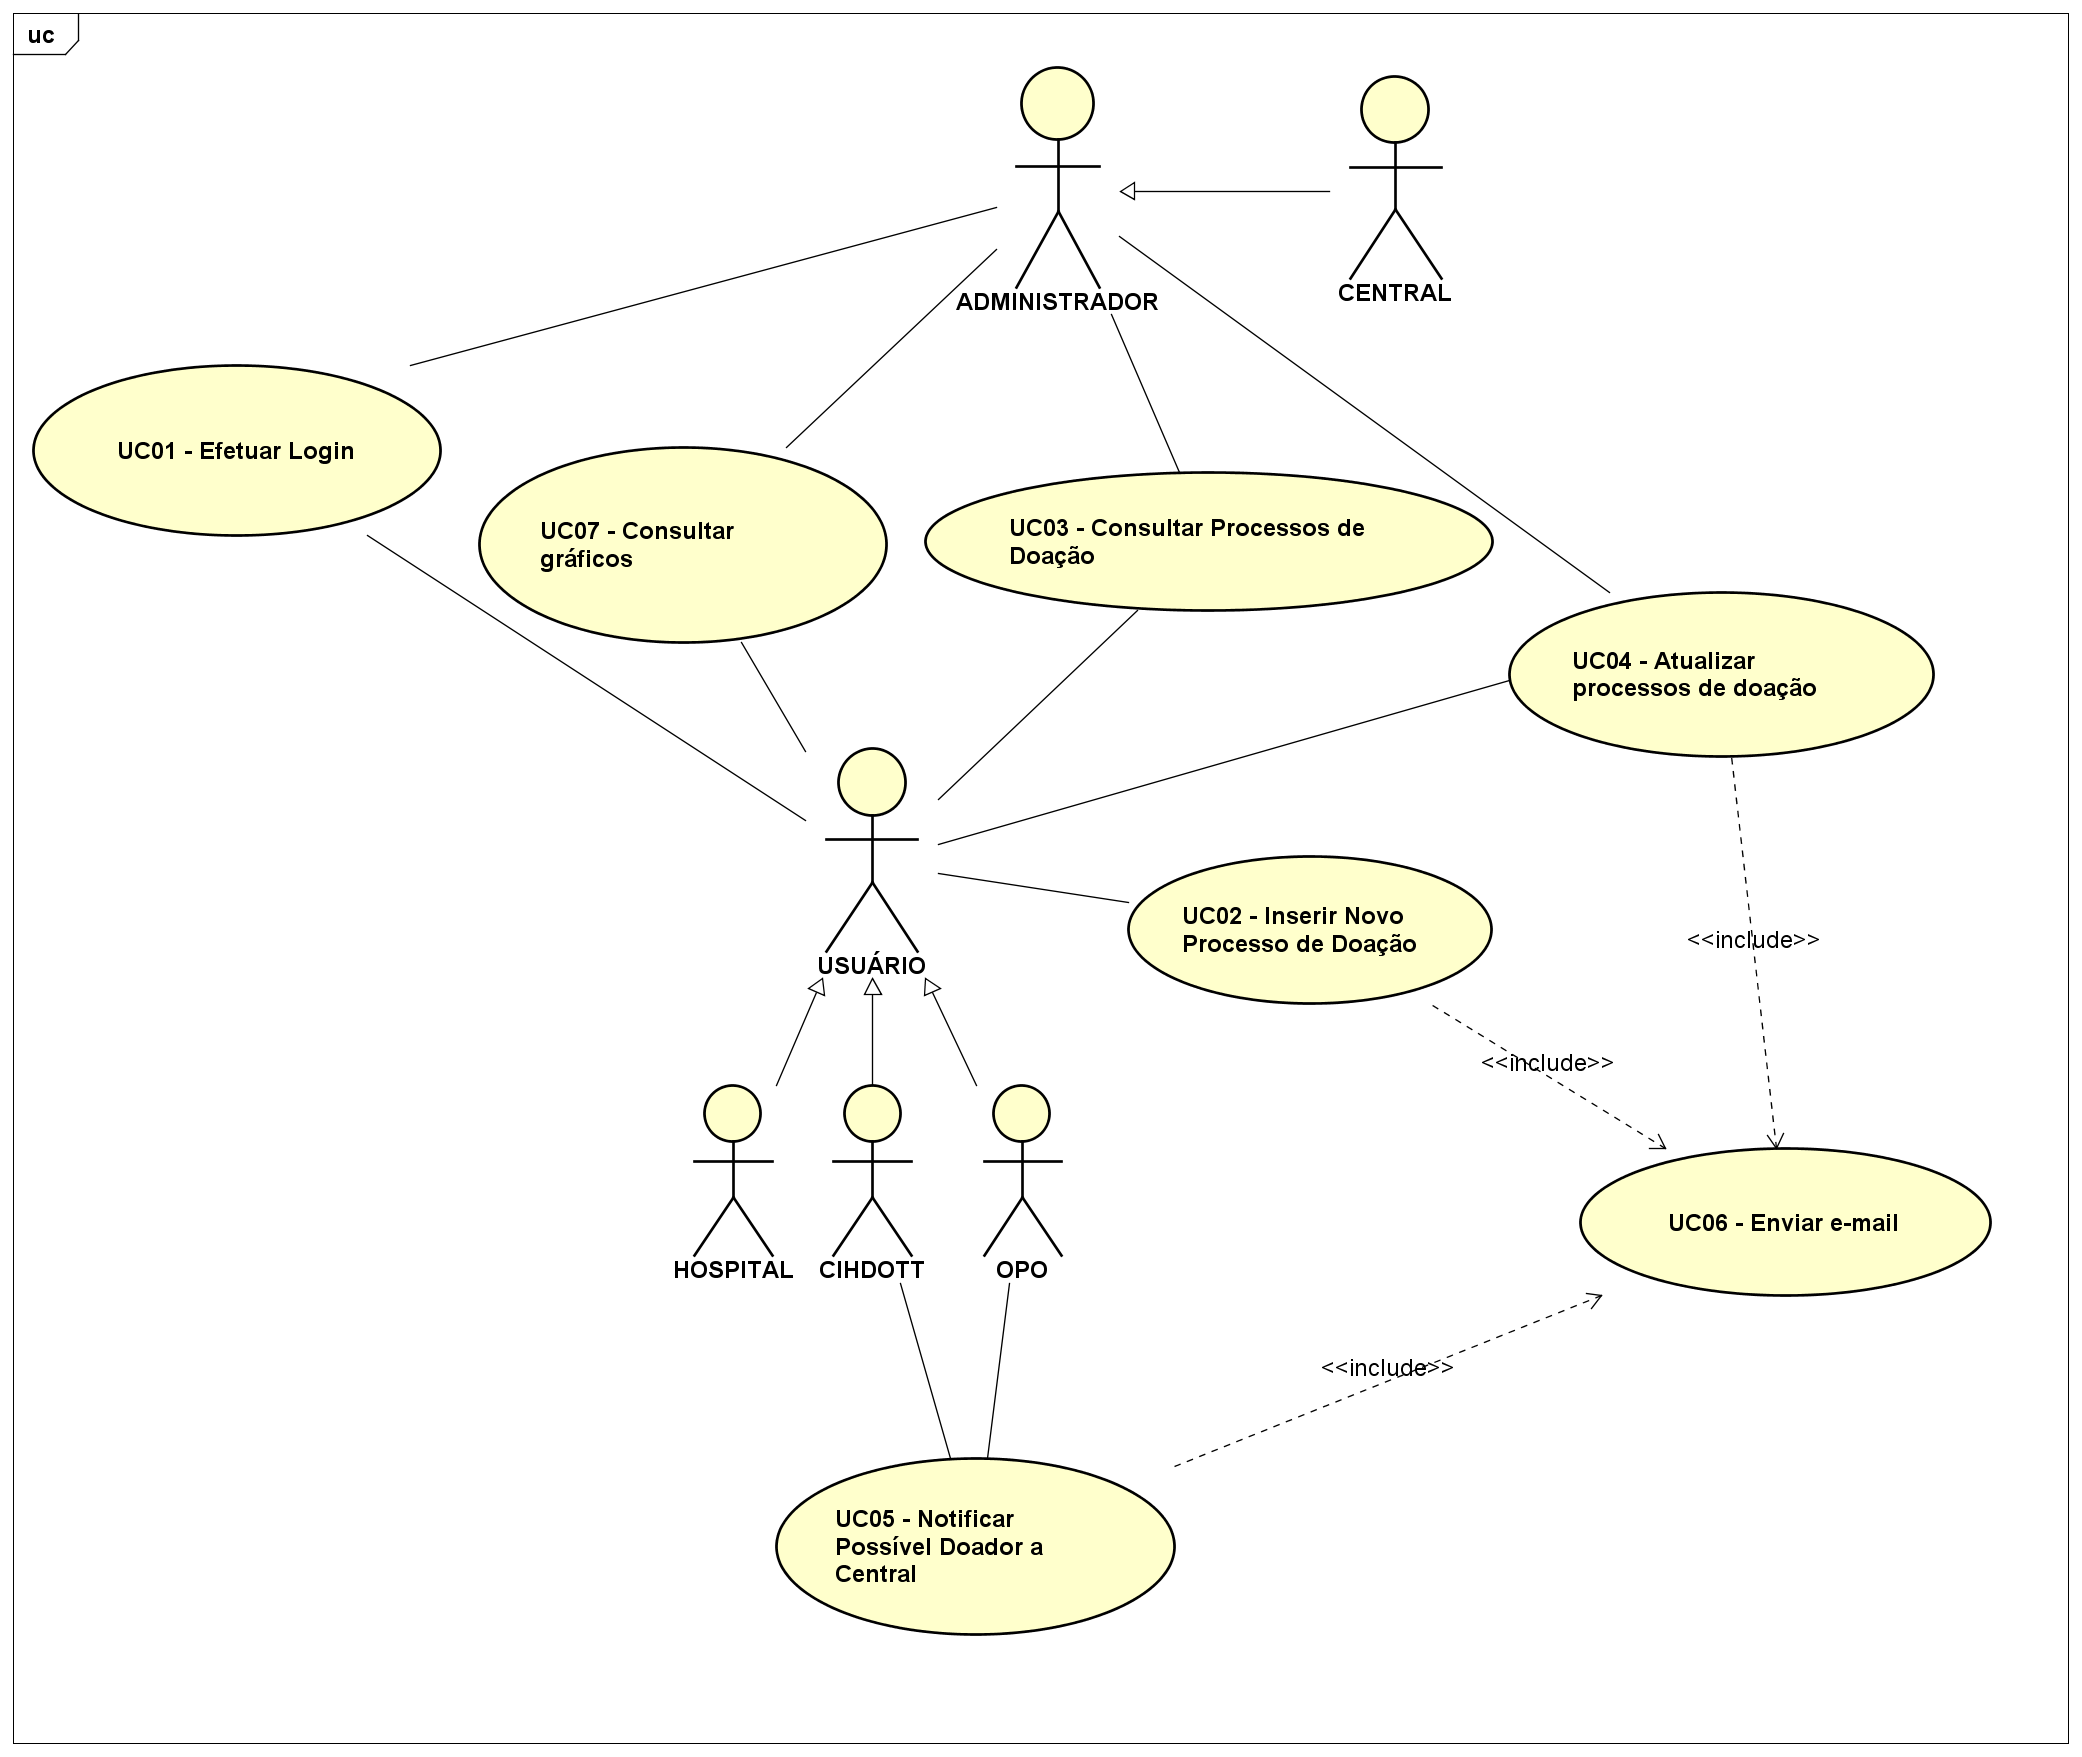
\includegraphics[width=17cm]{uc}
\label{fig:uc-diagram}
\end{figure}

\paragraph*{• UC01 - Efetuar Login}\label{tab:uc-login}
Para os atores Usuário e Administrador terem acesso as funcionalidades do software é necessário efetuar login com os dados obrigatórios descritos na Tabela \ref{table:uc01}.


%Efetuar Login
\begin{table}
  \centering
  \caption{UC01 - Efetuar Login} \label{table:uc01}
\begin{tabular}{ |p{5cm}|p{5cm}|  }
%\hline
%\multicolumn{2}{|c|}{UC01 - Efetuar Login} \\

%Atores
\hline
Atores & 
Administrador, Usuário \\

%Descrição
\hline
Descrição & 
Efetuar login no sistema. \\

%Dados Obrigatórios
\hline
Dados Obrigatórios & Usuário, Senha
 \\

%Dados não Obrigatórios
\hline
Dados não Obrigatórios & 
 \\

%Requisitos Relacionados
\hline
Requisitos Relacionados & RF01, RF03, RF06
 \\

\hline

\end{tabular}

\end{table}


%-------------------------------------
%UC02 - Inserir Novo Processo de Doação

\paragraph*{• UC02 - Inserir Novo Processo de Doação} \label{tab:uc-inserir}
Para o ator Usuário incluir um novo processo de doação e captação de órgãos no software é necessário fornecer os dados obrigatórios descritos na Tabela \ref{table:uc02}.

\begin{table}
	\centering
	\caption{UC02 - Inserir Novo Processo de Doação} \label{table:uc02}
		\begin{tabular}{ |p{5cm}|p{5cm}|  }
			%Atores
\hline
Atores & 
Usuário\\

%Descrição
\hline
Descrição & 
Cadastrar novo processo de doação no sistema. \\

%Dados Obrigatórios
\hline
Dados Obrigatórios & 
Hospital, Data Internação, Setor, Leito, Telefone, Informante, Nome, RG, CPF, CNS, Endereço, Filiação, Estado Civil, Telefone Familiar, Data de Nascimento, Idade, Sexo, Tipagem, Peso, Altura, Prontuário do Hospital, Causa da Morte, Decorrente De, Circunstância
 \\

%Dados não Obrigatórios
\hline
Dados não Obrigatórios & 

 \\

%Requisitos Relacionados
\hline
Requisitos Relacionados & 
RF02, RF03, RF04
 \\
 
 \hline
		\end{tabular}
\end{table}

%\newpage

%-------------------------------------
%UC03 - Consultar Processos de Doação

\paragraph*{• UC03 - Consultar Processos de Doação}
Para consultar os processos de doação e captação de órgãos no software os atores Usuário e Administrador podem fornecer os dados que não são obrigatórios conforme descrito na Tabela \ref{table:uc03}.

\begin{table}
\centering
\caption{UC03 - Consultar Processos de Doação} \label{table:uc03}
\begin{tabular}{ |p{5cm}|p{5cm}|  }
%\hline
%\multicolumn{2}{|c|}{UC03 - Consultar Processos de Doação} \\

%Atores
\hline
Atores & 
Administrador, Usuário\\

%Descrição
\hline
Descrição & 
 
Consultar processos de doação existente no sistema.
 \\

%Dados Obrigatórios
\hline
Dados Obrigatórios & 
 \\

%Dados não Obrigatórios
\hline
Dados não Obrigatórios & 
Nome, RG, CPF, Data
 \\

%Requisitos Relacionados
\hline
Requisitos Relacionados & 
RF02, RF03, RF06, RF09
 \\

\hline
\end{tabular}
\end{table}

%-------------------------------------
%UC04 - Atualizar Processos de Doação

\paragraph*{• UC04 - Atualizar Processos de Doação}
Para os atores Usuário e Administrador atualizarem os processos de doação e captação de órgãos no software é necessário fornecer os dados obrigatórios descritos na Tabela \ref{table:uc04}.

\begin{table}
\centering
\caption{UC04 - Atualizar Processos de Doação} \label{table:uc04}
\begin{tabular}{ |p{5cm}|p{5cm}|  }
%Atores
\hline
Atores & 
Administrador, Usuário\\

%Descrição
\hline
Descrição & 
 
Atualizar processos de doação existente no sistema.
 \\

%Dados Obrigatórios
\hline
Dados Obrigatórios & 
Hospital, Data Internação, Setor, Leito, Telefone, Informante, Nome, RG, CPF, CNS, Endereço, Filiação, Estado Civil, Telefone Familiar, Data de Nascimento, Idade, Sexo, Tipagem, Peso, Altura, Prontuário do Hospital, Causa da Morte, Decorrente De, Circunstância
 \\

%Dados não Obrigatórios
\hline
Dados não Obrigatórios & 
 \\

%Requisitos Relacionados
\hline
Requisitos Relacionados & 
RF02, RF03, RF07, RF11
 \\

\hline
\end{tabular}
\end{table}

%\newpage

%-------------------------------------
%UC05 - Notificar possível doador a Central

\paragraph*{• UC05 - Notificar possível doador a Central}
Para os atores CIHDOTT e OPO notificarem um doador de órgãos a Central Regional de Transplates é necessário fornecer os dados obrigatórios descristos na Tabela \ref{table:uc05}. 

\begin{table}
\centering
\caption{UC05 - Notificar possível doador a Central} \label{table:uc05}
\begin{tabular}{ |p{5cm}|p{5cm}|  }

%Atores
\hline
Atores & 
CIHDOTT, OPO\\

%Descrição
\hline
Descrição & 
 
Notificar possível doador a central de transplantes.
 \\

%Dados Obrigatórios
\hline
Dados Obrigatórios & 
Teste Clínico 1, Data, Hora, Nome do Médico
 \\

%Dados não Obrigatórios
\hline
Dados não Obrigatórios & 
 \\

%Requisitos Relacionados
\hline
Requisitos Relacionados & 
RF02, RF03, RF12
 \\

\hline

\end{tabular}
\end{table}


%-------------------------------------
%UC06 - Enviar e-mail

\paragraph*{• UC06 - Enviar e-mail}
Para o software enviar um e-mail a Central Regional de Transplantes é necessário que os atores insiram ou atualizem um processo respeitando os dados obrigatórios descritos na Tabela \ref{table:uc06}. 

\begin{table}
\centering
\caption{UC06 - Enviar e-mail} \label{table:uc06}
\begin{tabular}{ |p{5cm}|p{5cm}|  }
%Atores
\hline
Atores & 
Administrador, Usuário\\

%Descrição
\hline
Descrição & 
 
Enviar e-mail a Central Regional de Transplantes
 \\

%Dados Obrigatórios
\hline
Dados Obrigatórios & 
Hospital, Data Internação, Setor, Leito, Telefone, Informante, Nome, RG, CPF, CNS, Endereço, Filiação, Estado Civil, Telefone Familiar, Data de Nascimento, Idade, Sexo, Tipagem, Peso, Altura, Prontuário do Hospital, Causa da Morte, Decorrente De, Circunstância
 \\

%Dados não Obrigatórios
\hline
Dados não Obrigatórios & 

 \\

%Requisitos Relacionados
\hline
Requisitos Relacionados & 
RF02, RF03, RF12
 \\

\hline
\end{tabular}
\end{table}

%\newpage

%-------------------------------------
%UC07 - Consultar gráficos

\paragraph*{• UC07 - Consultar gráficos}
Para consultar os gráficos que o software fornece os atores Administrador e Usuário precisam estar logados conforme descrito na Tabela \ref{table:uc07}. 

\begin{table}
\centering
\caption{UC07 - Consultar gráficos} \label{table:uc07}
\begin{tabular}{ |p{5cm}|p{5cm}|  }

%Atores
\hline
Atores & 
Administrador, Usuário\\

%Descrição
\hline
Descrição & 
 
Consultar gráficos dos processos no sistema.
 \\

%Dados Obrigatórios
\hline
Dados Obrigatórios & Estar logado no sistema
 \\

%Dados não Obrigatórios
\hline
Dados não Obrigatórios & 
 \\

%Requisitos Relacionados
\hline
Requisitos Relacionados & 
RF02, RF03, RF05
 \\

\hline

\end{tabular}
\end{table}


\section{Diagrama Entidade Relacionamento}
Esta seção apresenta e descreve o Modelo Entidade Relacionamento representado pela figura \ref{fig:erDiagram}, onde se pode ver todas entidades envolvidas com seus atributos e relacionamentos.

\begin{figure}[htp]
\centering
\caption{Diagrama Entidade Relacionamento}
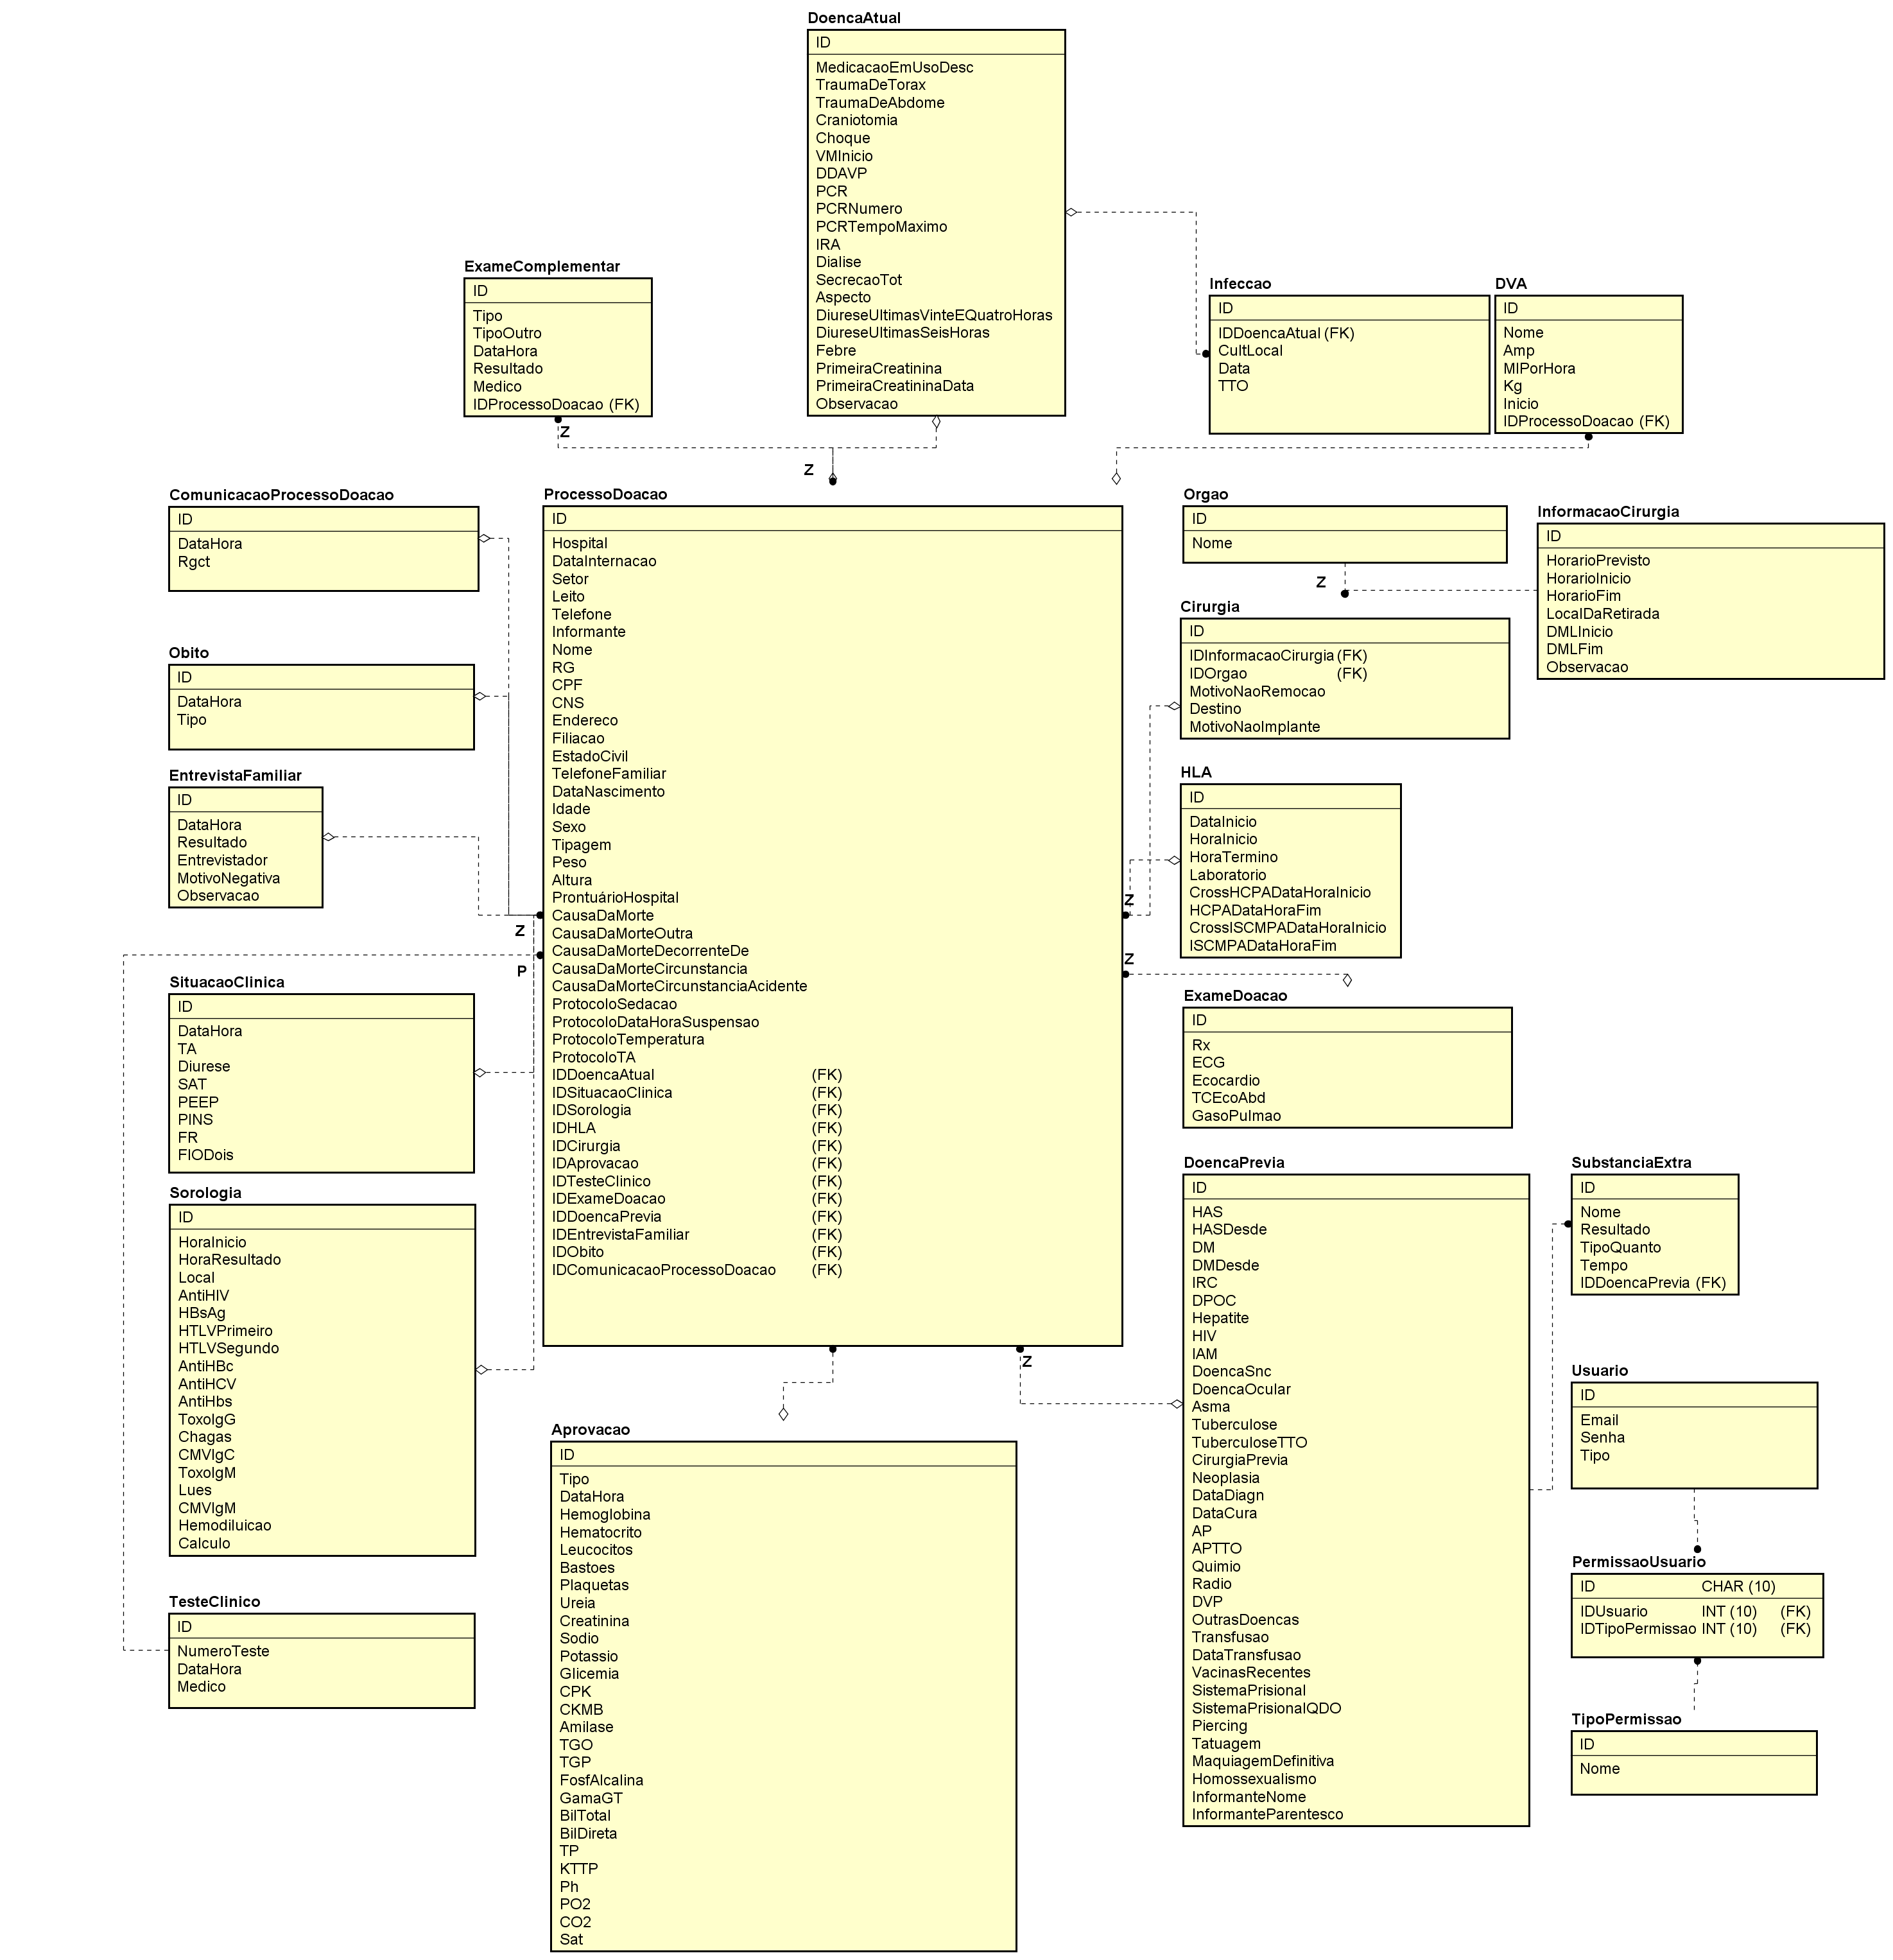
\includegraphics[width=15cm]{er-diagram}
\label{fig:erDiagram}
\end{figure}

\newpage

\paragraph*{• Processo Doação}
A entidade \textit{ProcessoDoacao} é utilizada para representar o processo de doação com informações pessoais do paciente, e relaciona-se com as entidades necessárias para representar o processo de captação e doação de órgãos.

\paragraph*{• Exame Complementar}
A entidade \textit{ExameComplementar} é utilizada para representar os exames complementares que o paciente deve realizar para iniciar o processo de captação e doação de órgãos.

\paragraph*{• Doença Atual}
A entidade \textit{DoencaAtual} é utilizada para representar as possíveis doenças que o paciente possa ter durante o processo de captação e doação de órgãos.

\paragraph*{• Infecção}
A entidade \textit{Infeccao} é utilizada para representar todas as infecções que o paciente tem.

\paragraph*{• DVA}
A entidade \textit{DVA} é utilizada para representar todas deficiências de vitamina A que o paciente tem, e então o médico decidir se a cirurgia pode ser realizada.

\paragraph*{• Órgão}
A entidade \textit{Orgao} é utilizada para representar todos os órgãos que podem ser doados.

\paragraph*{• Informação Cirurgia}
A entidade \textit{InformacaoCirurgia} é utilizada para representar os dados gerais para se realizar uma cirurgia tais como horário inicial, final e outras informações.

\paragraph*{• Cirurgia}
A entidade \textit{Cirurgia} é utilizada para representar todas as cirurgias  de transplante, junto com as informações gerais e quais os órgãos que estão sendo transplantados.

\paragraph*{• HLA}
A entidade \textit{HLA} é utilizada para representar todos os testes para avalia a compatibilidade entre o doador e o receptor.

\paragraph*{• Exame Doação}
A entidade \textit{ExameDoacao} é utilizada para representar os cinco exames necessários antes de realizar a cirurgia no paciente.

\paragraph*{• Doença Prévia}
A entidade \textit{DoencaPrevia} é utilizada para representar todas as doenças do paciente antes de realizar a cirurgia.

\paragraph*{• Substância Extra}
A entidade \textit{SubstanciaExtra} é utilizada para representar as substâncias que o paciente possa ter adquirido antes de realizar a cirurgia.

\paragraph*{• Aprovação}
A entidade \textit{Aprovacao} é utilizada para representar as substâncias que precisam ser verificadas e autorizadas quando o paciente da entrada no hospital. 

\paragraph*{• Teste Clínico}
A entidade \textit{TesteClinico} é utilizada para representar dois testes clínicos obrigatórios antes de comunicar a central de transplantes.

\paragraph*{• Sorologia}
A entidade \textit{Sorologia} é utilizada para representar o diagnóstico e a identificação de anticorpos e antígenos no soro do paciente.

\paragraph*{• Situação Clínica}
A entidade \textit{SituacaoClinica} é utilizada para representar a situação clínica do paciente que é medida através dos atributos listados na entidade.

\paragraph*{• Entrevista Familiar}
A entidade \textit{EntrevistaFamiliar} é utilizada para representar a entrevista realizada junto a família do paciente.

\paragraph*{• Óbito}
A entidade \textit{Obito} é utilizada para representar informações básicas do óbito do paciente que estão listadas na entidade.

\paragraph*{• Comunicação Processo Doação}
A entidade \textit{ComunicacaoProcessoDoacao} é utilizada para representar a comunicação entre a Central Regional de Órgãos e a Central Nacional de Órgãos.

\paragraph*{• Usuário}
A entidade \textit{Usuario} é utilizada para representar as informações dos usuários do software de captação e doação de órgãos. 

\paragraph*{• Tipo Permissão}
A entidade \textit{TipoPermissao} é utilizada para representar as permissões existentes no software de captação e doação de órgãos.

\paragraph*{• Permissão Usuário}
A entidade \textit{PermissaoUsuario} é utilizada para representar as permissões de cada usuário cadastrado no software de captação e doação de órgãos.

\section{Diagrama de Classe}
Este capítulo apresenta o diagrama de classe para o desenvolvimento do software de captação e doação de órgãos que é representado pela Figura \ref{fig:erDiagram}.

\begin{figure}[htp]
\centering
\caption{Diagrama de Classe}
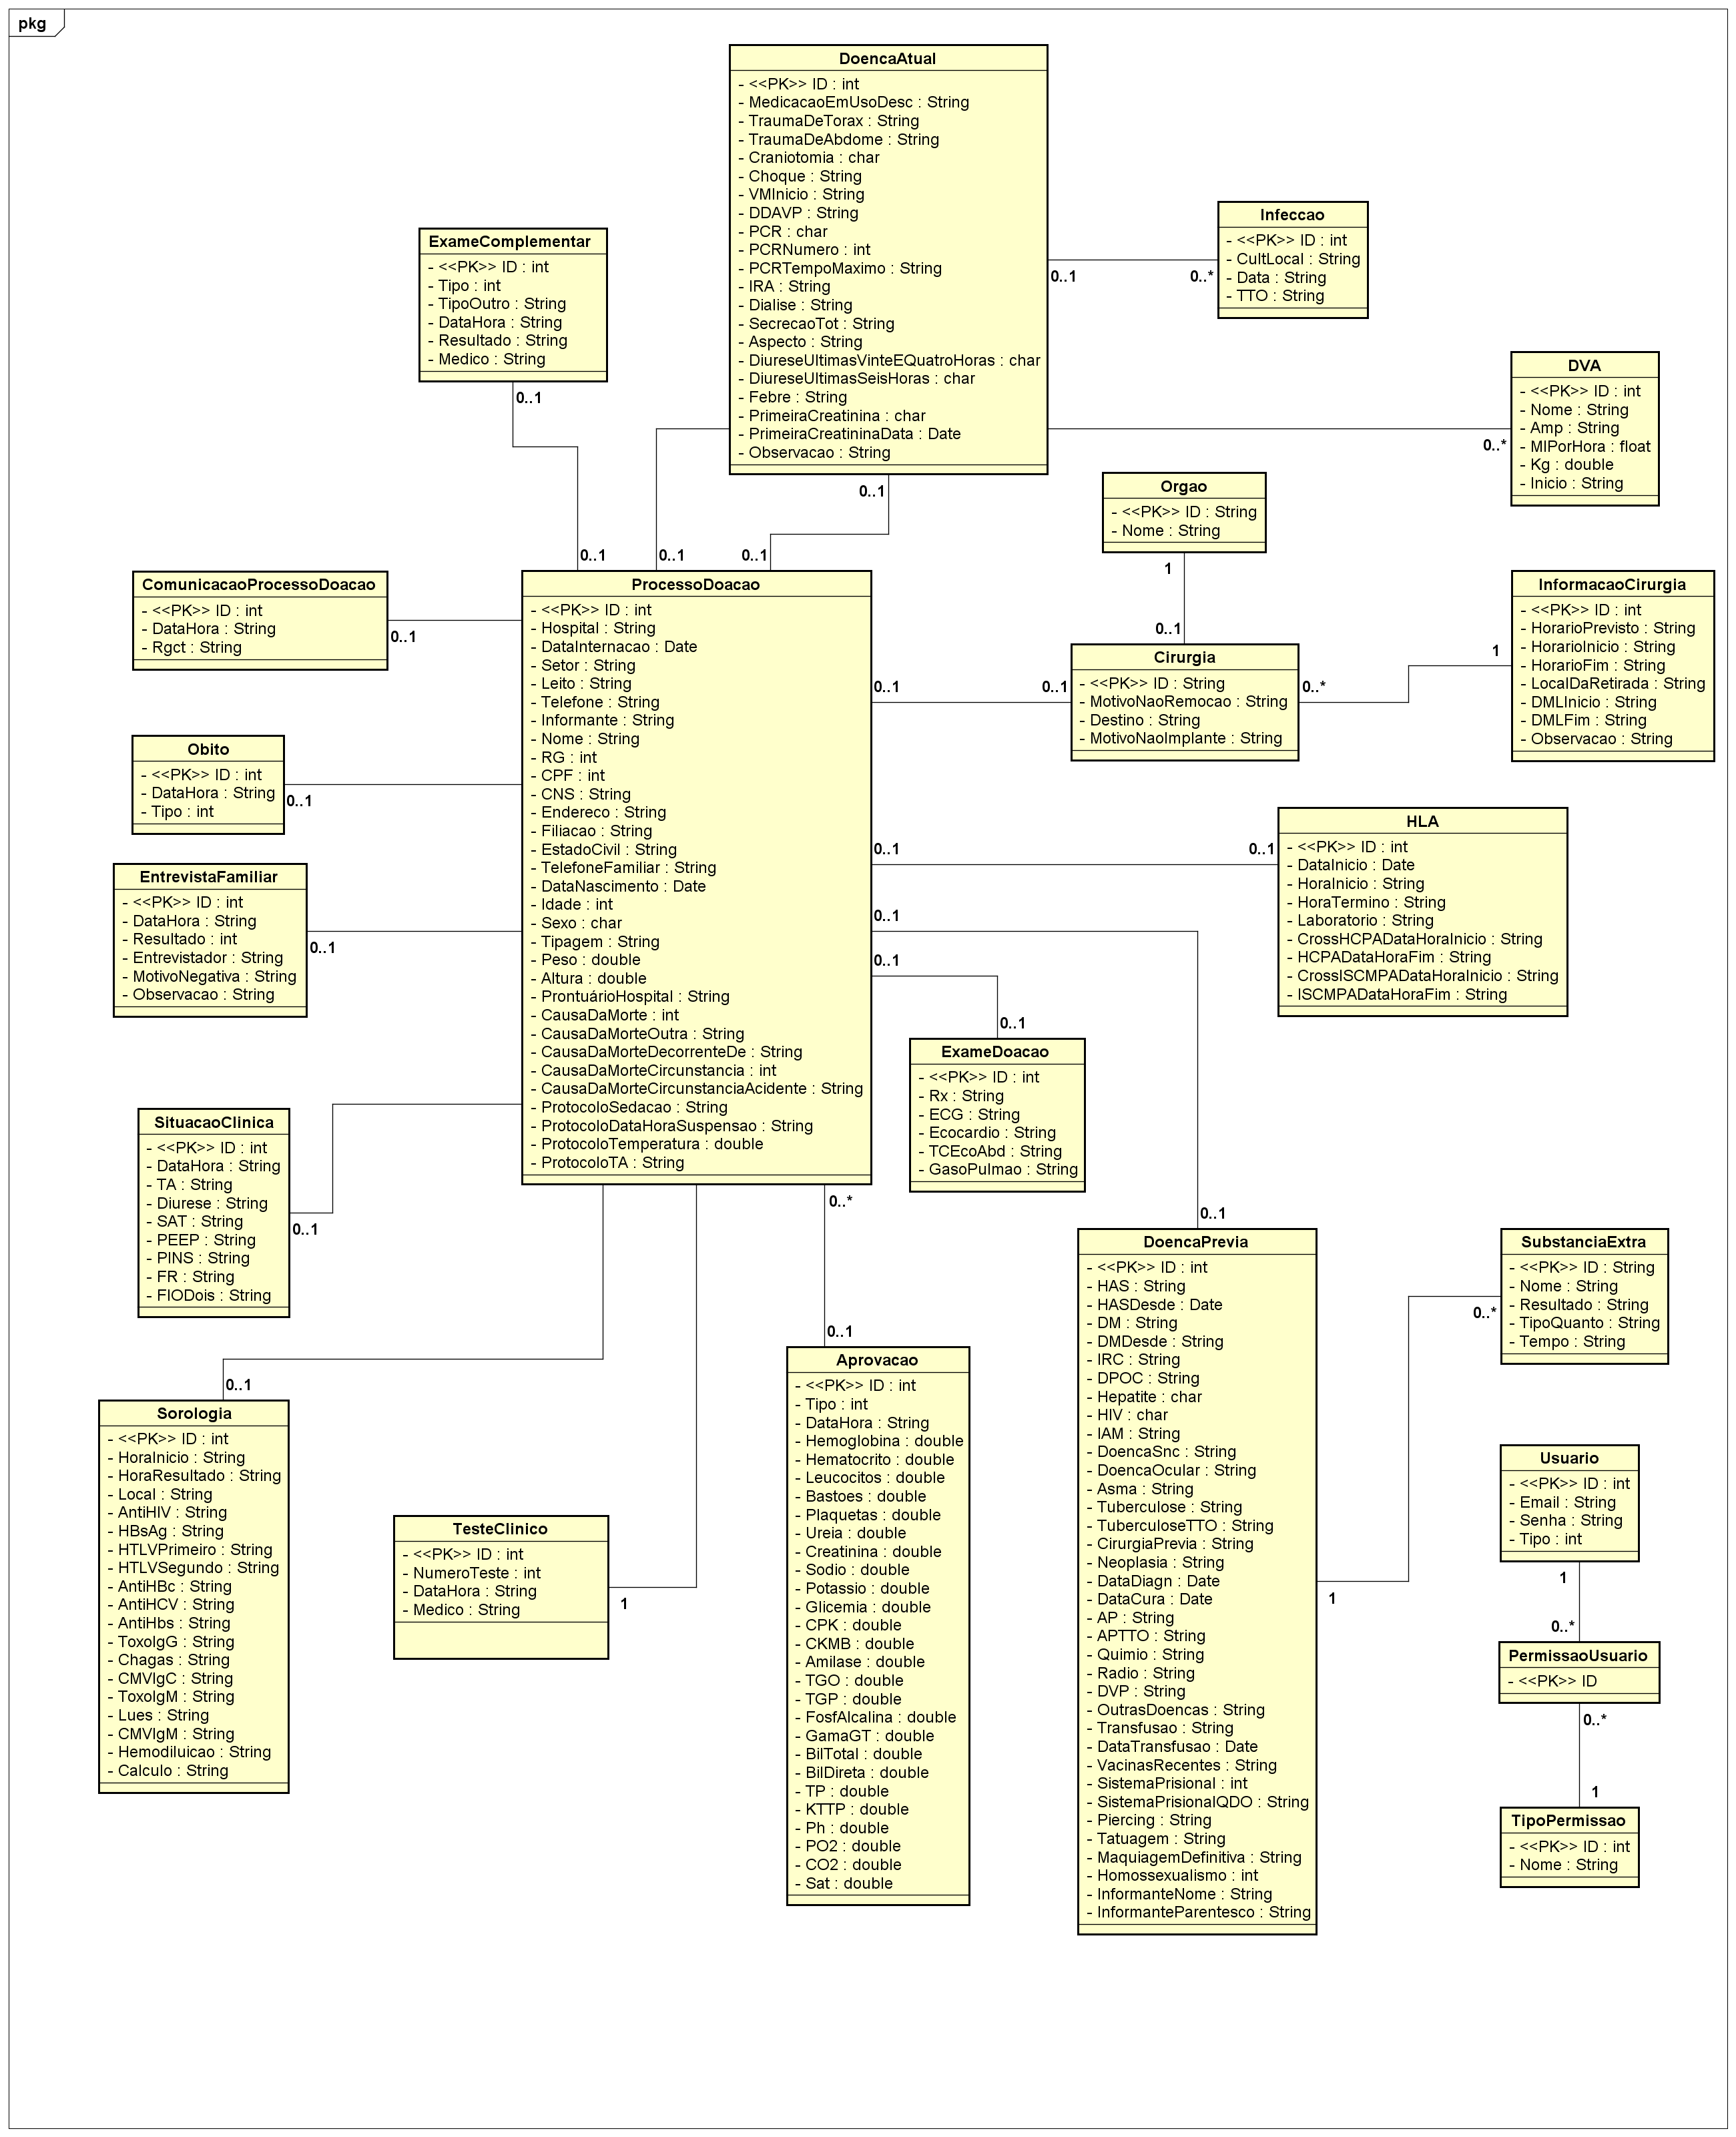
\includegraphics[width=15cm]{class-diagram}
\label{fig:erDiagram}
\end{figure}

\chapter{Protótipo}
Este capítulo apresenta e descreve as principais telas do aplicativo móvel, onde os usuários interagem junto a plataforma proposta; É importante salientar que os dados preenchido nas telas são fictícios.

\section{FLORENCE: Tela de Login}
A Figura \ref{fig:app-login} apresenta a tela de login no aplicativo móvel para usuários e administradores conforme descrito na Seção \ref{tab:uc-login}.

\begin{figure}[htp]
\centering
\caption{FLORENCE: Tela de Login}
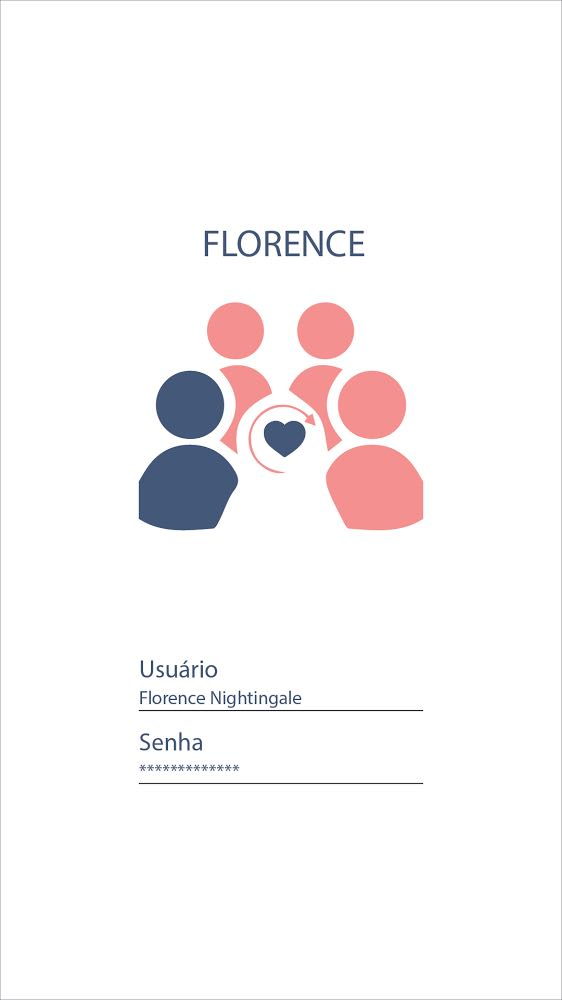
\includegraphics[width=6cm]{app-login}
\label{fig:app-login}
\end{figure}

Nesta tela o usuário deve preencher seu usuário e senha para então o software autenticar se o usuário preenchido existe. Se o usuário existir esta tela é redirecionada para a tela de listagem dos processos.  



%\newpage

\section{FLORENCE: Tela para Criação de Processo}
A Figura \ref{fig:app-criacao} apresenta a tela de criação de um novo processo com os dados básicos do paciente, dados estes que são obrigatórios conforme descrito na Seção \ref{tab:uc-inserir}.

\begin{figure}[htp]
\centering
\caption{FLORENCE: Tela para Criação de Processo}
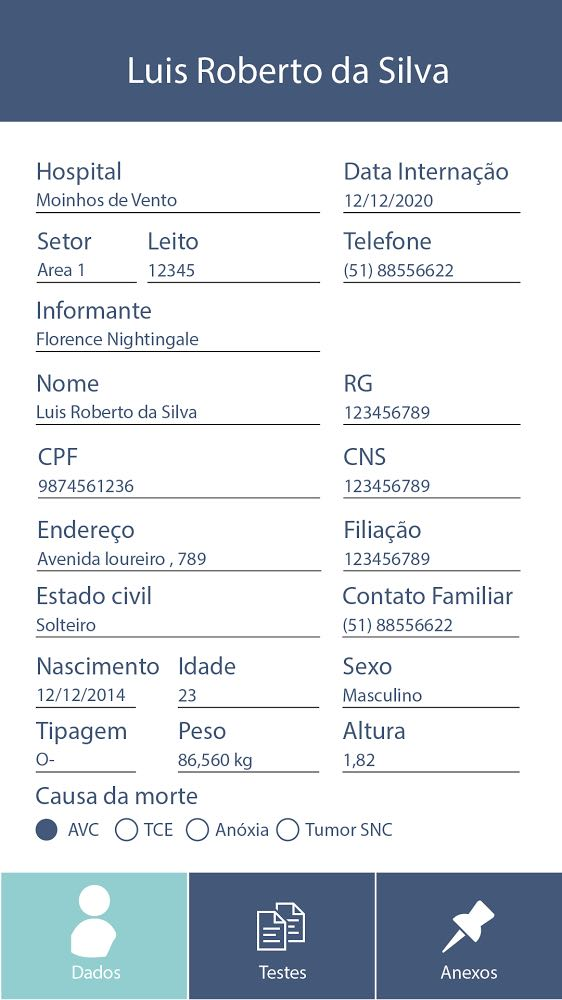
\includegraphics[width=6cm]{app-data}
\label{fig:app-criacao}
\end{figure}

Nesta tela o usuário terá a opção de incluir ou editar os dados básicos do paciente, testes clínicos ou anexos vinculados ao processo.

%\newpage

\section{FLORENCE: Tela de Anexo}
A Figura \ref{fig:app-anexo} apresenta a tela com todos os arquivos anexados junto ao processo do paciente.

\begin{figure}[htp]
\centering
\caption{FLORENCE: Tela para Anexar Documentos}
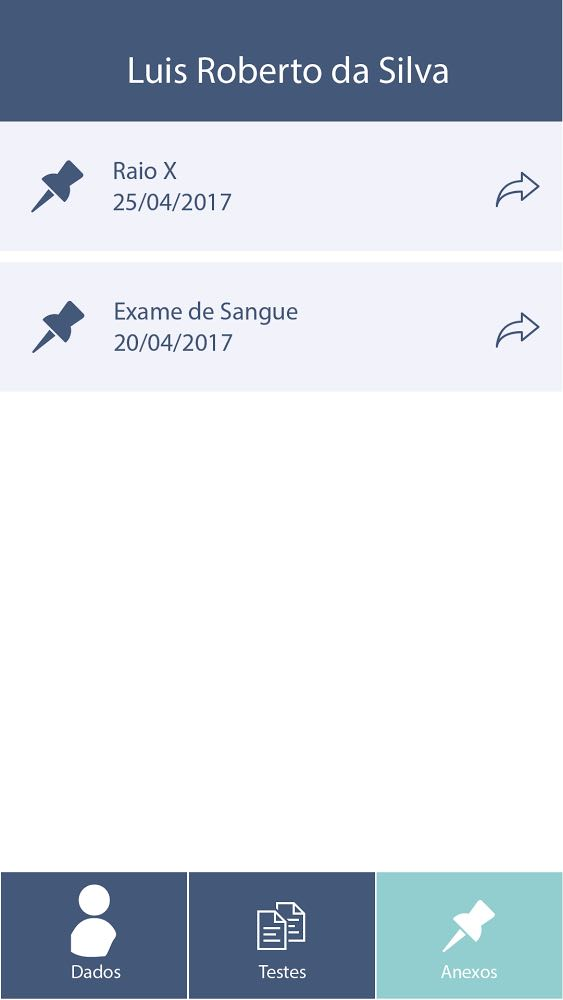
\includegraphics[width=5cm]{app-attachment}
\label{fig:app-anexo}
\end{figure}

Nesta tela o usuário pode pode incluir ou editar os documentos vinculados ao processo; Nesta tela o usuário tem a opção de ir para a tela de Dados ou Testes.

%\newpage

\section{FLORENCE: Tela De Listagem dos Processos}
A Figura \ref{fig:app-list} apresenta a tela com a lista de todos os processos vinculados ao usuário logado.

\begin{figure}[htp]
\centering
\caption{FLORENCE: Tela para listagem dos Processos}
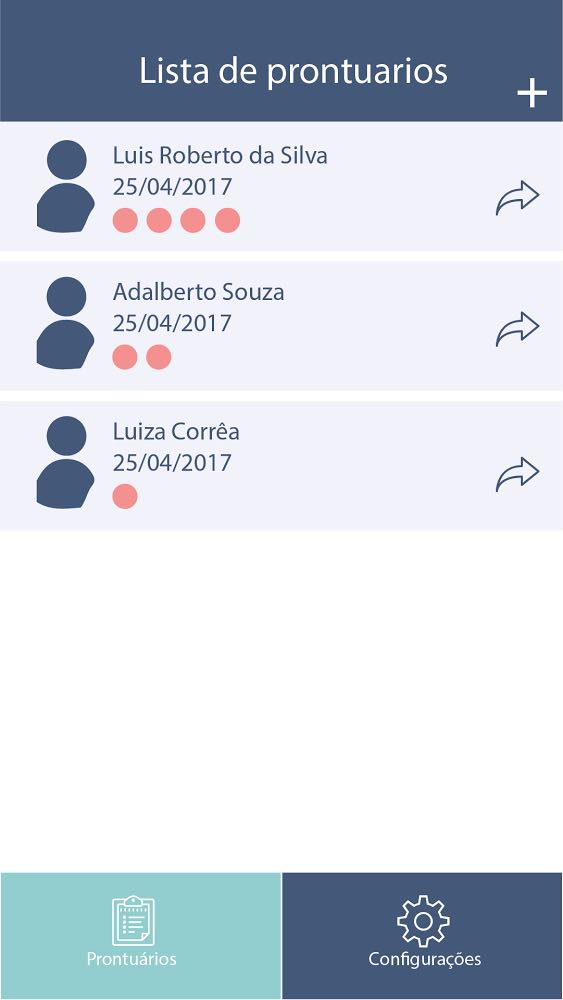
\includegraphics[width=6cm]{app-list}
\label{fig:app-list}
\end{figure}

Nesta tela o usuário tem a opção de selecionar um dos processos e visualizar os dados básicos do paciente, testes clínicos e os documentos anexados.
%\newpage

\section{FLORENCE: Tela de Configuração}

\begin{figure}[htp]
\centering
\caption{FLORENCE: Tela de Configuração}
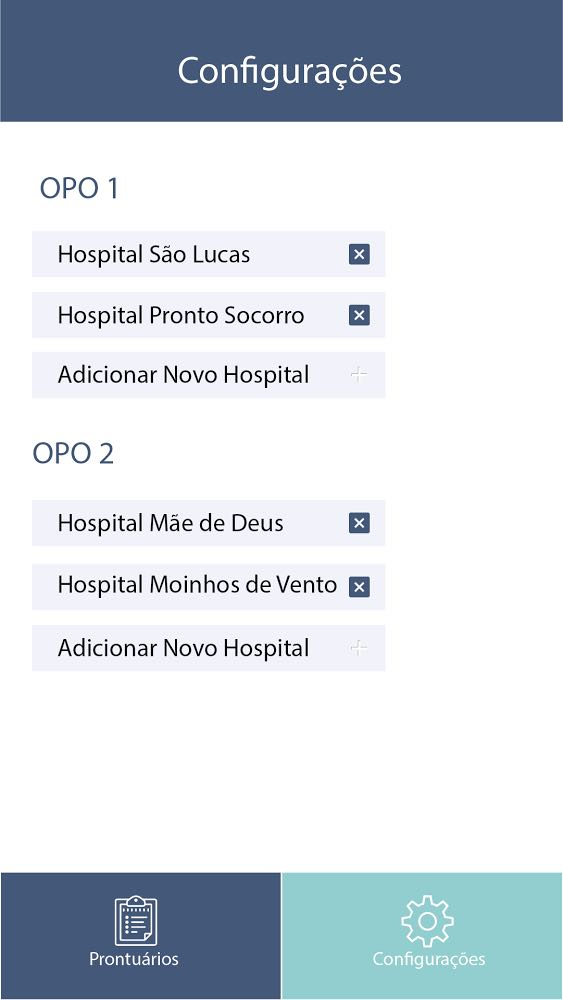
\includegraphics[width=6cm]{app-config}
\label{fig:app-config}
\end{figure}

A Figura \ref{fig:app-config} apresenta a tela para configurar os hospitais de cada OPO que só pode ser acessada por um usuário Administrador. 

\chapter{Descrição das Atividades}
Para o desenvolvimento do software proposto, esta seção descreve um cronograma das atividades necessárias conforme o Capítulo \ref{tab:descricao-trabalho}.

\begin{ganttchart}[y unit title=0.4cm,
  y unit chart=0.8cm,
  vgrid,hgrid,
  title label anchor/.style={below=-1.6ex},
  title left shift=.05,
  title right shift=-.05,
  title height=1,
  bar/.style={fill=gray!50},
  incomplete/.style={fill=white},
  progress label text={},
  bar height=0.7,
  group right shift=0,
  group top shift=.6,
  group height=.3,
  group peaks height={.2}
  ]{1}{24}
  \gantttitle{2017}{24} \\ 
  \gantttitle{Jul}{4}
  \gantttitle{Ago}{4}
  \gantttitle{Set}{4}
  \gantttitle{Out}{4}
  \gantttitle{Nov}{4}
  \gantttitle{Dez}{4} \\
  %tasks
  \ganttbar{1}{3}{6} \\ %ambiente
  \ganttbar{2}{7}{17} \\ %desenvolvimento
  \ganttbar{3}{13}{19} \\ %test
  \ganttbar{4}{3}{19} \\ %escrita
  \ganttbar{5}{20}{21} \\ %apresentacao

  %relations
 % \ganttlink{elem0}{elem1}
 % \ganttlink{elem1}{elem2}
 % \ganttlink{elem2}{elem3}
 % \ganttlink{elem3}{elem4}
 % \ganttlink{elem4}{elem5}
 % \ganttlink{elem5}{elem6}
 % \ganttlink{elem6}{elem7}

\end{ganttchart}


\paragraph*{1 - Configuração de Ambiente}
Nesta estapa será configurado o ambiente local de desenvolvimento com a configuração da nuvem, banco de dados e estrutura do código fonte.

\paragraph*{2 - Desenvolvimento}
Nesta etapa será desenvolvido o software para captação e doação de órgãos conforme descrito no Capítulo \ref{tab:descricao-trabalho}.

\paragraph*{3 - Teste}
Nesta etapa serão realizados testes funcionais e de integração no software.

\paragraph*{4 - Escrita TCC}
Nesta etapa será escrito toda a segunda etapa do trabalho de conclusão.

\paragraph*{5 - Apresentação}
Nesta etapa será apresentado a solução junto a banca do trabalho de conclusão.


\chapter{Conclusão}
Concluímos que os principais problemas tecnológicos enfrentados pelas entidades envolvidas no processo de doação de órgãos são as inconsistências e a segurança dos dados. 
 
Através de uma plataforma hospedada em uma nuvem privada, garantindo um melhor tratamento de confidencialidade nos dados, a plataforma a ser desenvolvida será capaz de revolucionar o processo atual de doação órgãos agregando um melhor controle de acesso e confidencialidade aos dados do paciente.

%\cite{NAGAPACKING07}
%\cite{CORMEMALGORITHMS01}
%\cite{SKIENAC698}
%\cite{BENTLEYBC07}
%\cite{BRIANPL04}
%\cite{OLIVEIRAAPL08}
%\cite{PICCOLIAPL11}
%\cite{PICCOLIDM08}
%\cite{GOLDENBERGAPL02}
%\cite{PLASSPAG81}

%\cite{XIAOAPL05}
%\cite{COFFMANPACKING98}
%\cite{WIKIPIC09}

%----------------------------------------------------------------
% Aqui vai a bibliografia. Existem 3 estilos de citação: use
% 'tcc-alpha' para citações do tipo [Abc+] ou [XYZ] (em ordem
% alfabética na bibliografia), 'tcc-num' para citações
% numéricas do tipo [1], [20], etc., em ordem de referência e
% 'tcc-alpha-full' para citações estilo 'alpha' mas com nomes completos.
%----------------------------------------------------------------

\bibliographystyle{tcc-alpha-full}
\bibliography{reference}

\end{document}
